%=== Préambule ===========================================================

\documentclass{beamer}
\usepackage{pdfpages}
\usepackage[english]{babel}
\usepackage{xspace}
\usepackage{pifont}
\usepackage{hyperref}
\usepackage{listings}
\usepackage{csquotes}
\usepackage{graphicx}
\usepackage{animate,media9} %,movie15}
\usepackage{wrapfig}
\usepackage{pdfpages}
\usepackage{tikz}
\usepackage{natbib}
\uselanguage{English}
\usepackage{fontawesome5}
\languagepath{English}
\setcounter{tocdepth}{1}
\usepackage{setspace}
\usepackage{amsmath}
\def\glasses{{\sffamily 
\leavevmode\rlap{%
\rotatebox[origin=tr]{125}{J}\kern1ex%  
\rotatebox[origin=tr]{125}{J}}% 
\rotatebox[origin=c]{-90}{D}%   
\rotatebox[origin=c]{-90}{D}}%
\def\ialy{\sffamily 
\resizebox{1ex}{1.5ex}{\reflectbox{\rotatebox[origin=]{75}{J}}}\kern-1pt%
\rlap{\tiny$\ ^\bullet\kern2.5pt^\bullet$ }%
\rotatebox[origin=c]{-90}{D}%   
\rotatebox[origin=c]{-90}{D}\kern-1pt%  
\resizebox{1ex}{1.5ex}{\rotatebox[origin=]{75}{J}}}}


\lstset{
  numbers=left,
  basicstyle=\tiny\ttfamily,      
  breaklines=true, 
  showtabs=false,
  showstringspaces=false,
}  

%=== Configuration de Beamer et du thème metropolis ======================
\usepackage{bbding}
\usetheme[background=light]{metropolis}
\usepackage[clock]{ifsym}

\definecolor{mLightBrown}{HTML}{000000}
\definecolor{black}{HTML}{000000}
\setbeamercolor{structure}{fg=black,bg=mLightBrown}
\setbeamercolor{palette primary}{%
	use=normal text,
	fg=normal text.bg,
	bg=mLightBrown
}
%\setsansfont[BoldFont={Linux Libertine G Bold},Numbers={OldStyle}]{Linux Libertine G}

\metroset{block=fill}

%=== Page de titre =======================================================

%path to logo and biblio -> to be adapted to your local directories 
\newcommand\dirlogo{../../logos/}
\newcommand\dirbiblio{../../biblio}



\title{{\normalsize \vskip 1cm Mission au P\'erou}}
\subtitle{\small 5-21 November 2022}
\author{Hugo S. \\ {\tiny Institut de Recherche pour le Développement IRD - ISTerre} \\ 
\\
Team : \\
Virginie Pinel, Hugo S\'anchez-Reyes, L\'ea Pousse, Bertrand Lovery\\
\\
\textit{Seminars at IGP (Instituto Geof\'isico del Per\'u), LabEx OSUG}
}

\date[2022]{\today}

\subject{Group Meeting}

\titlegraphic{\centering \vspace{-18pt}
\includegraphics[height=1.2cm]{../../../logos/logo_seminar_2022.pdf} \par} %\qquad  
\includegraphics[height=1.4cm]{../../logos/anr_eqtime.png} \par }


\addtobeamertemplate{frametitle}{}{%
\begin{tikzpicture}[remember picture,overlay]
  \node[anchor=north east,yshift=0.0ex] at (current page.north east) {
\includegraphics[height=4ex]{../../logos/ISTerre_neg.pdf}};
  %\node[anchor=north east,yshift=0.5ex] at (current page.north east) {\includegraphics[height=3.3ex]{\dirlogo/seiscope_color_light_background}};
\end{tikzpicture}}



%=== Document ============================================================

\begin{document}


\begin{frame}
 \titlepage
\end{frame}

\begin{frame}

 {Outline}
  \tableofcontents
  
\end{frame}



\section{Arequipa}
 

 \begin{frame}
  
  {Tasks}
  
  5 Days course of INSAR ... 8:30h to 17:00h
  \vskip 0.5cm \pause
  \begin{itemize}
   \item Adquisition \pause
   \item Preprocessing \pause
   \item Corrections \pause
   \item Time series analysis \pause
   \item Volcanic monitoring \pause
   \item Volcanic source modeling \pause
   \item Sentinel missions \pause
   \item FlatSim project \pause
   \item UGA Master Programs \pause
  \end{itemize}

  Virginie (main teacher), L\'ea and Bertrand (teaching assistants), Hugo (official translator and amazing student!)

  
 \end{frame}

 
 \begin{frame}
 
 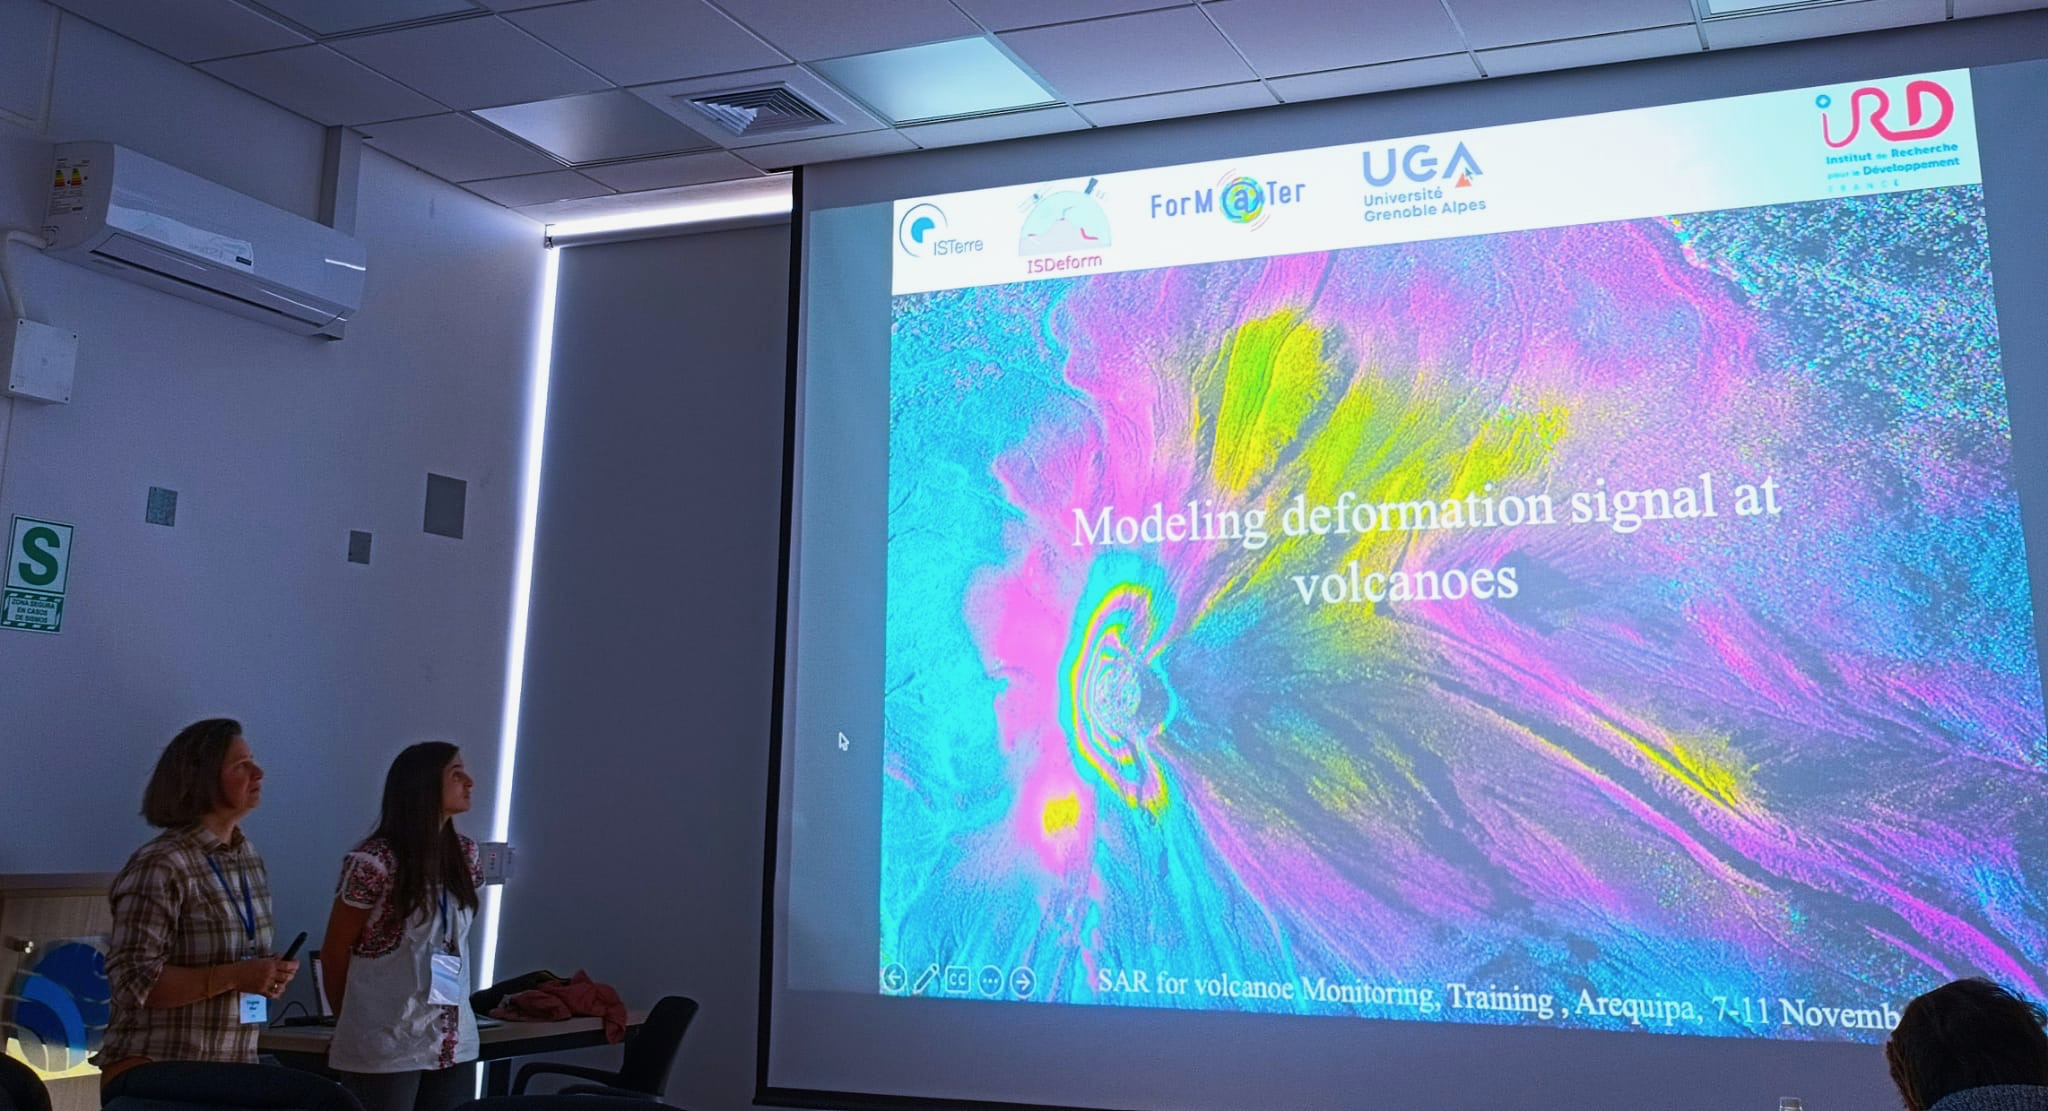
\includegraphics[width=1\linewidth]{images/CoursVirginieLéa.jpeg}
 
\end{frame}



\begin{frame}
 
 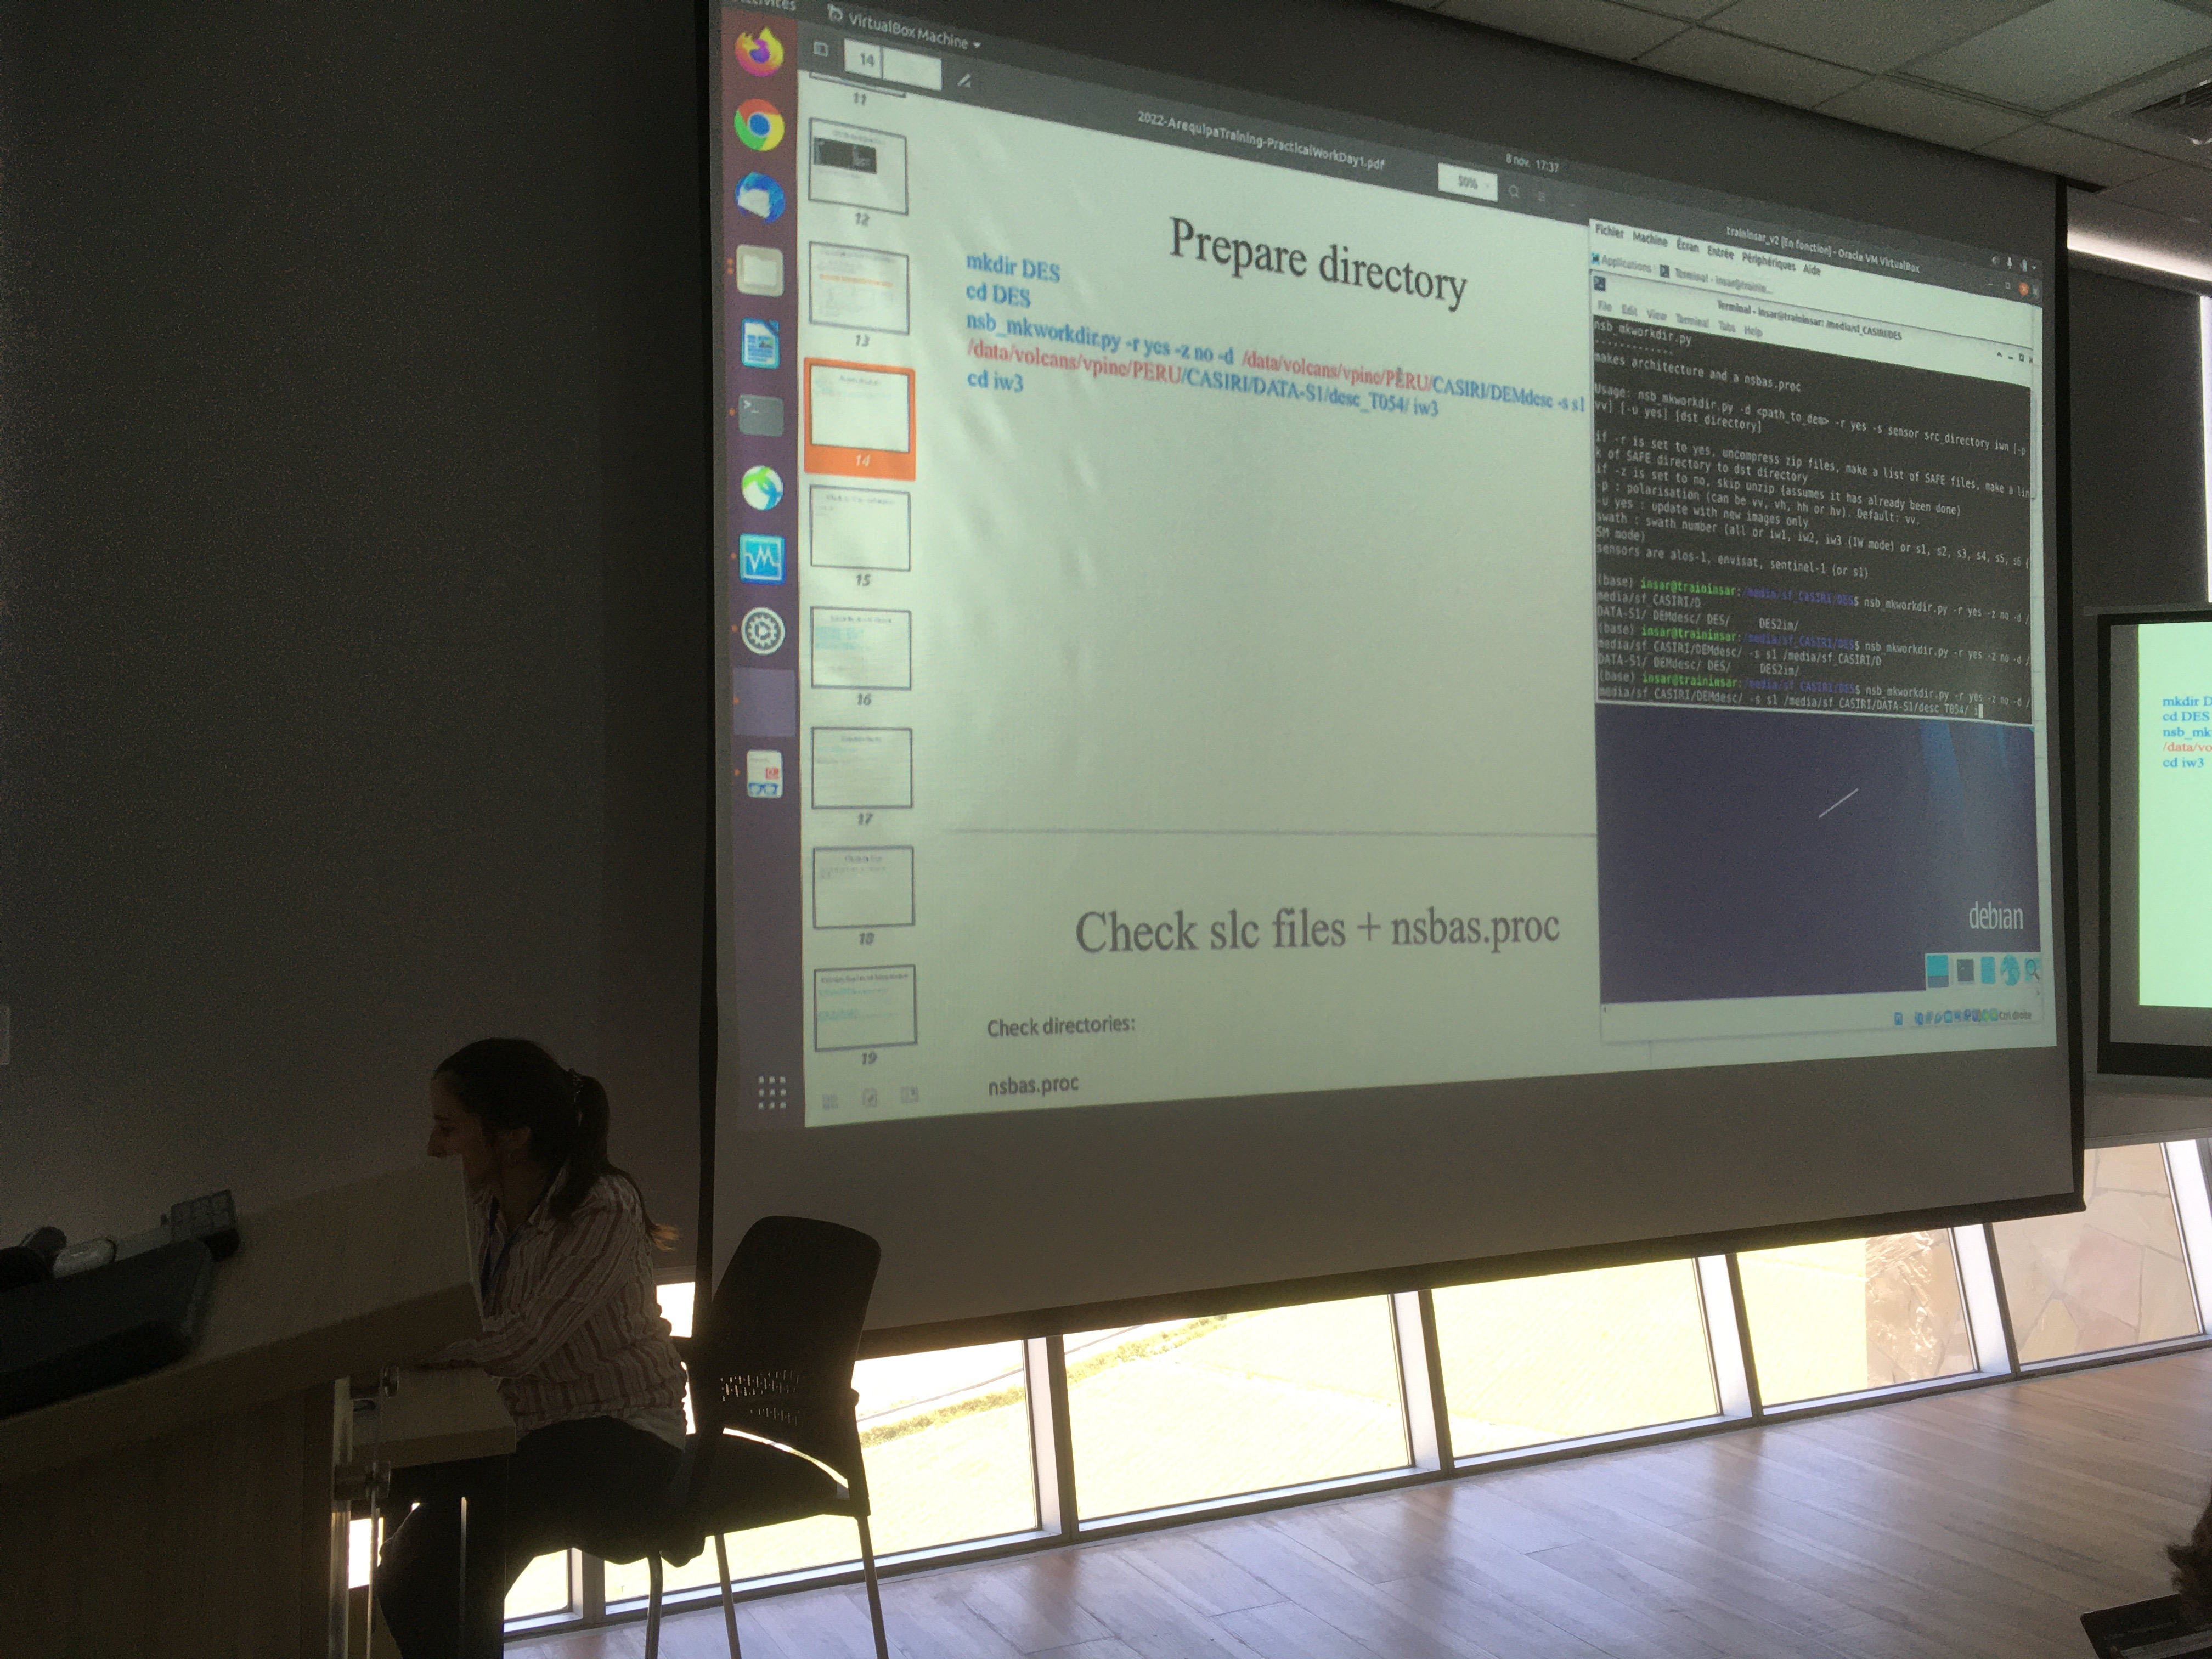
\includegraphics[width=1\linewidth]{images/CoursLea.jpeg}
 
\end{frame}


\begin{frame}
 
 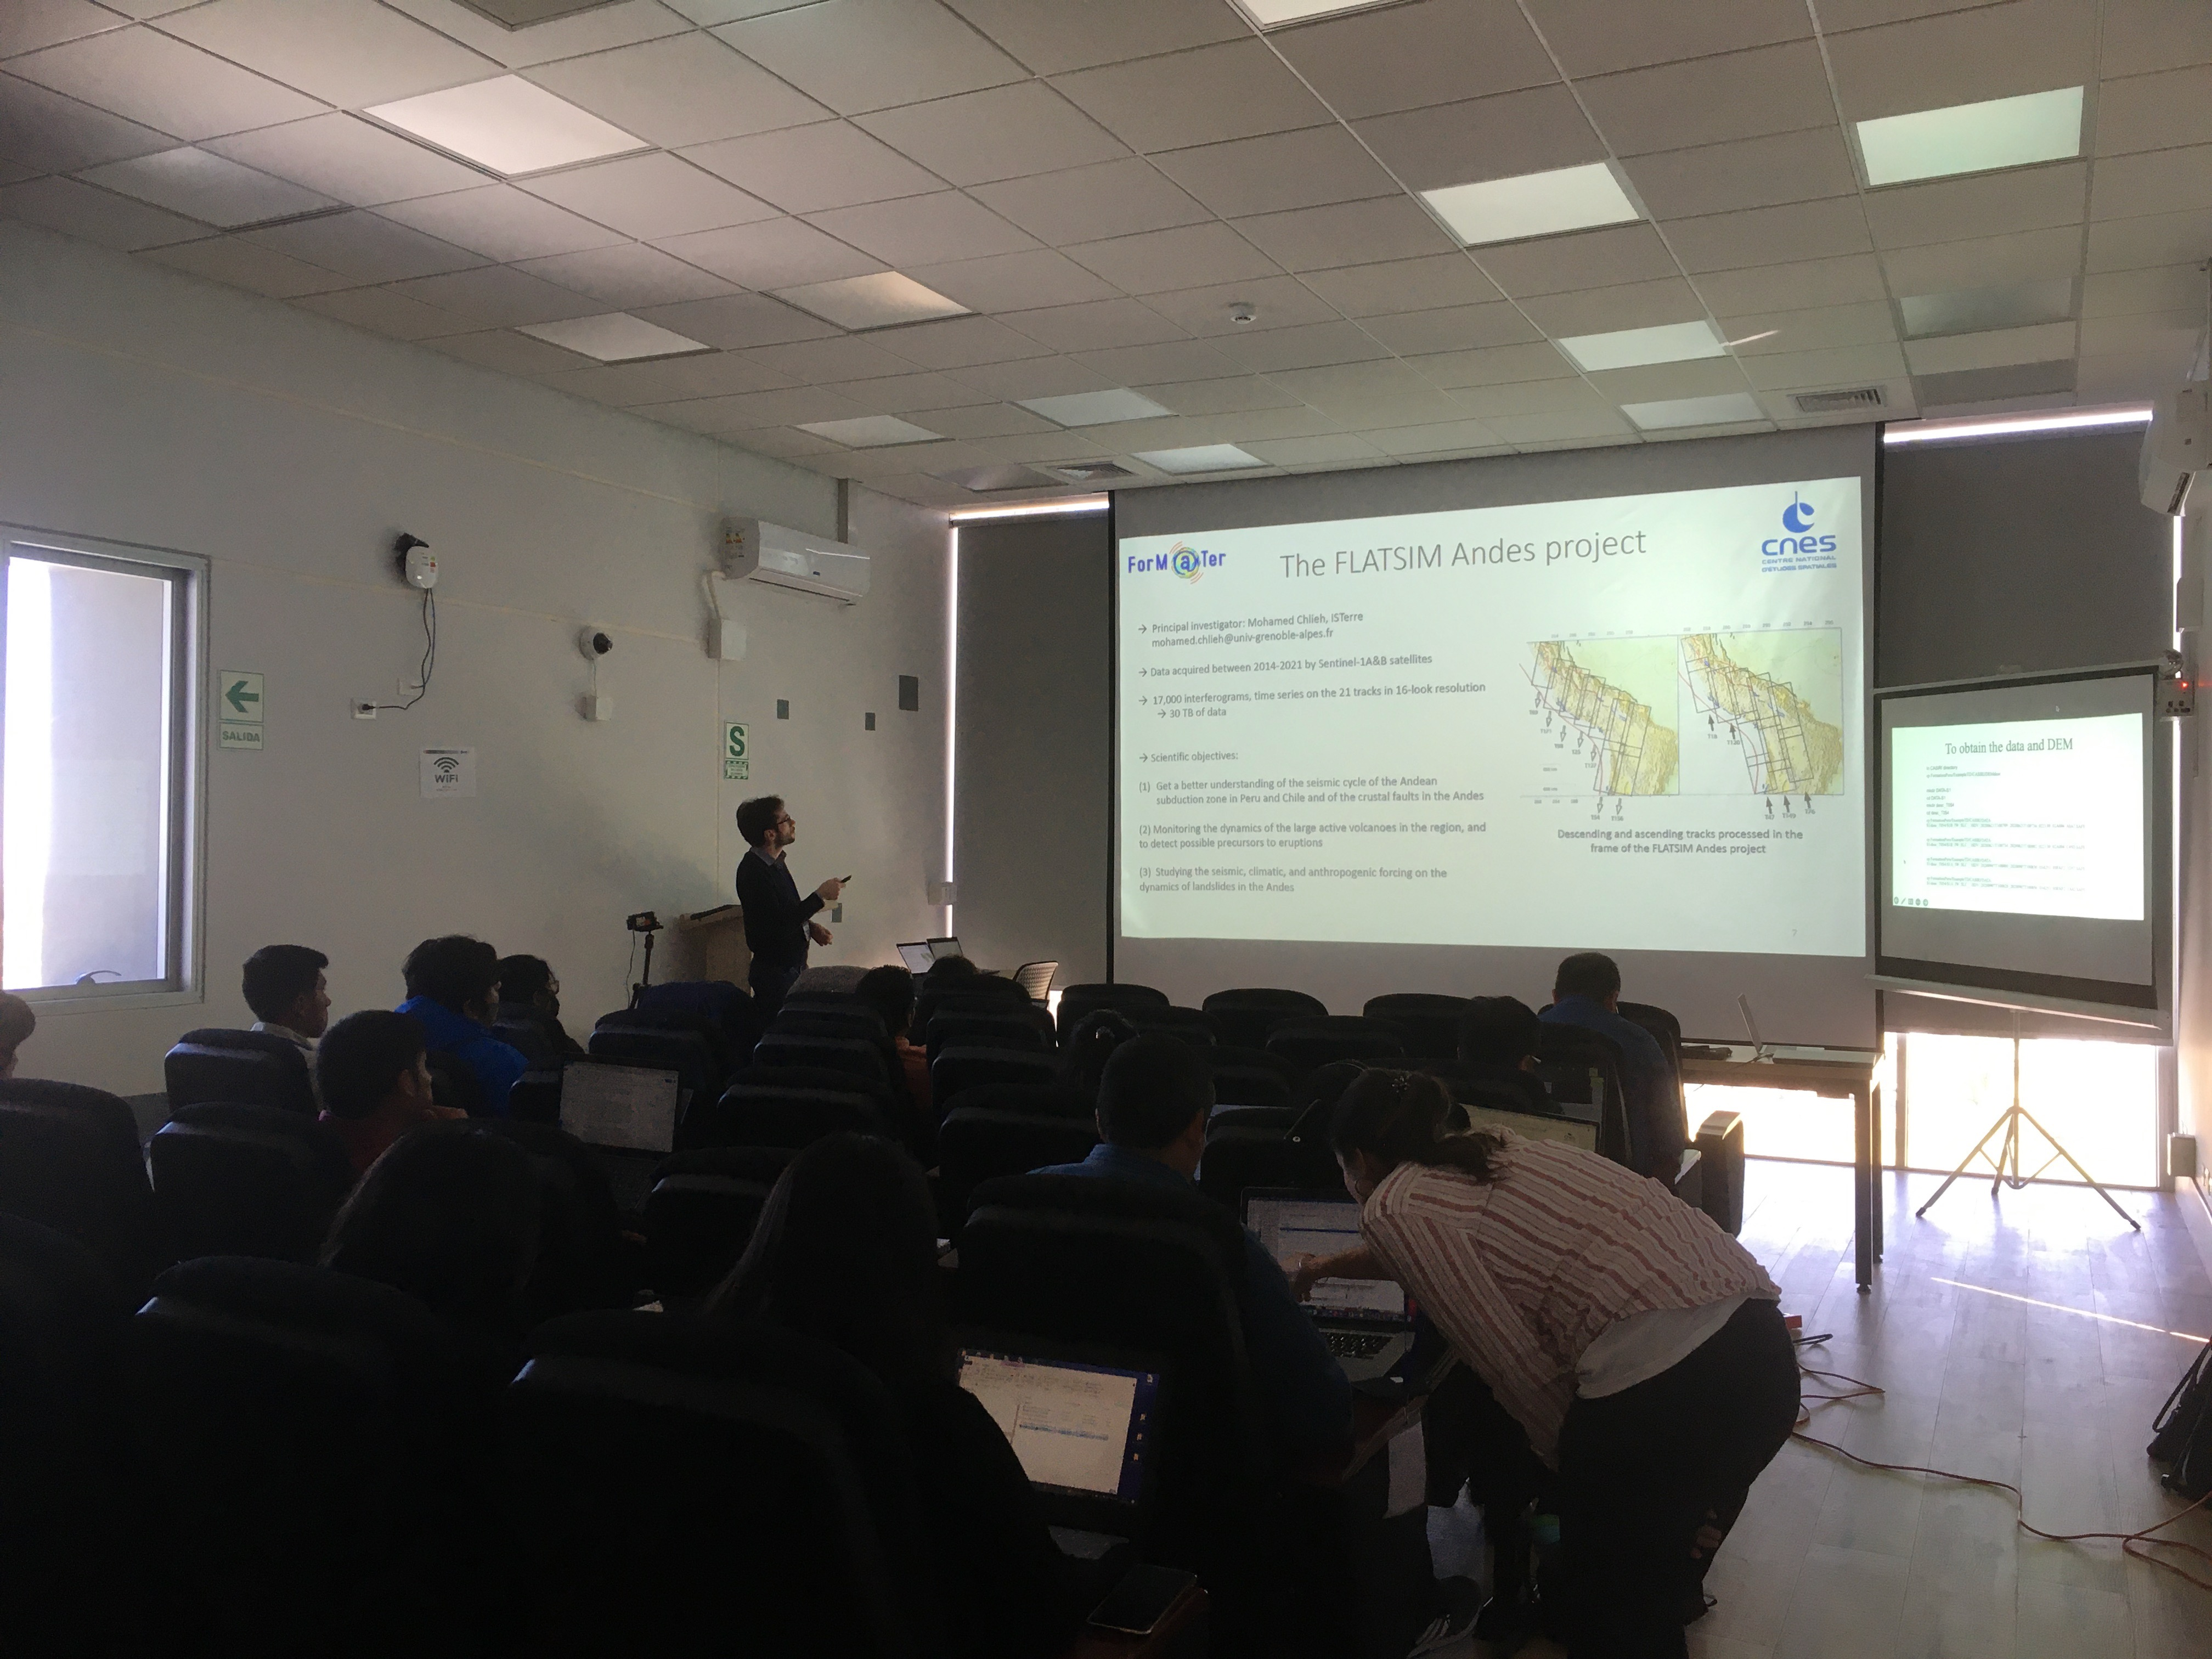
\includegraphics[width=1\linewidth]{images/CoursBertrand.jpeg}
 
\end{frame}


\begin{frame}
 
 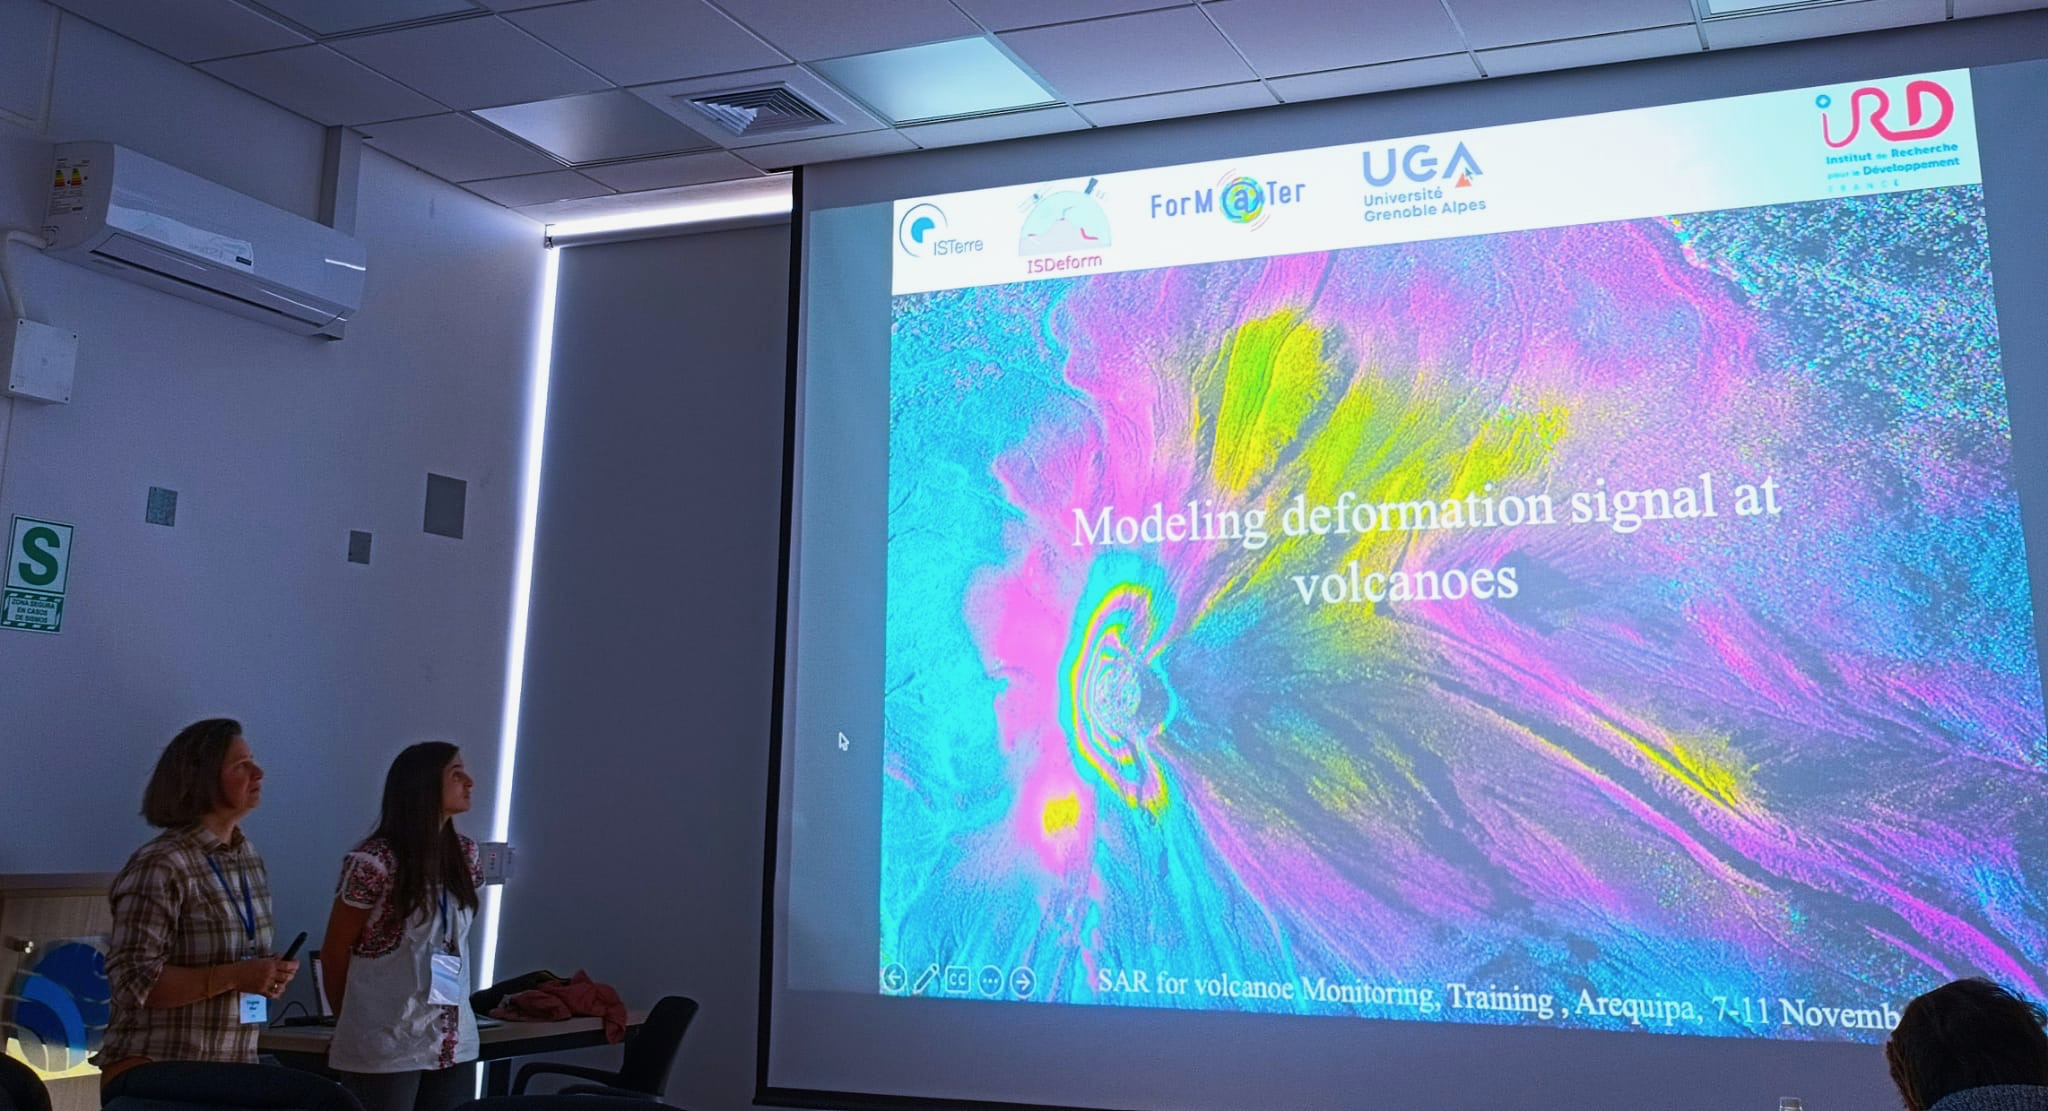
\includegraphics[width=1\linewidth]{images/CoursVirginieLéa.jpeg}
 
\end{frame}


\begin{frame}
 
 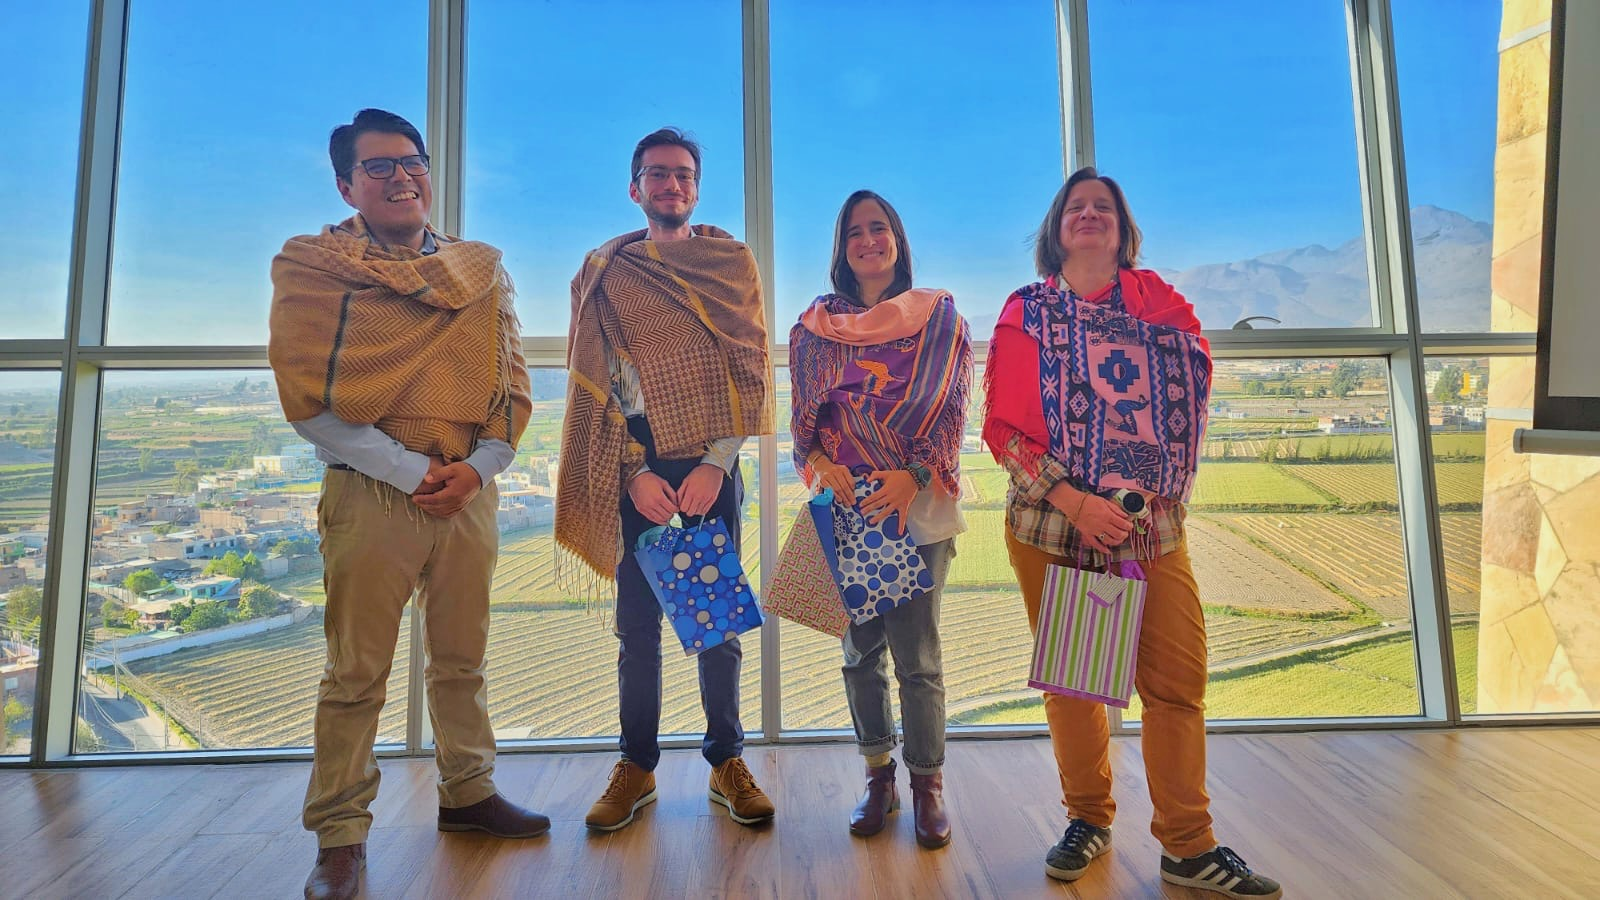
\includegraphics[width=1\linewidth]{images/KdoIGPGroupeBest.jpeg}
 
\end{frame}


\begin{frame}

 {All participants}
 
 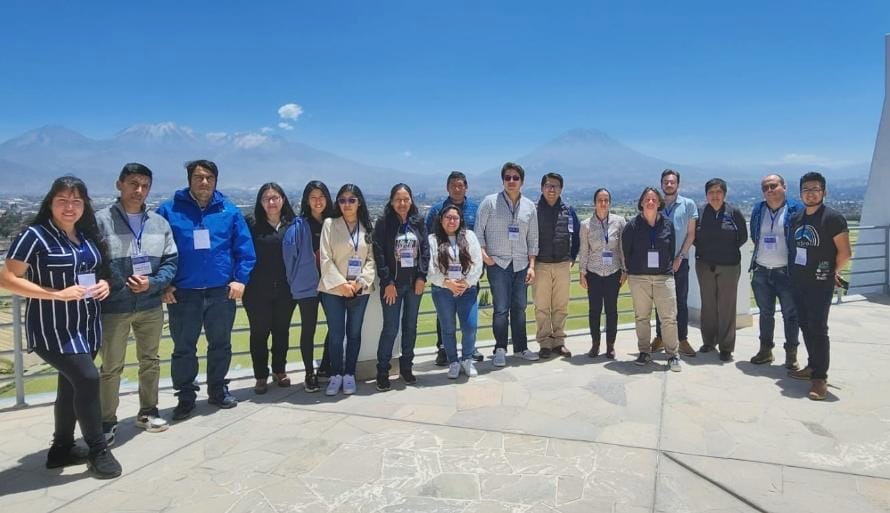
\includegraphics[width=1\linewidth]{images/GroupeTotalTerrasse.jpeg}
 
\end{frame}


\begin{frame}
 
 {IGP web site news}
 
 \centering
 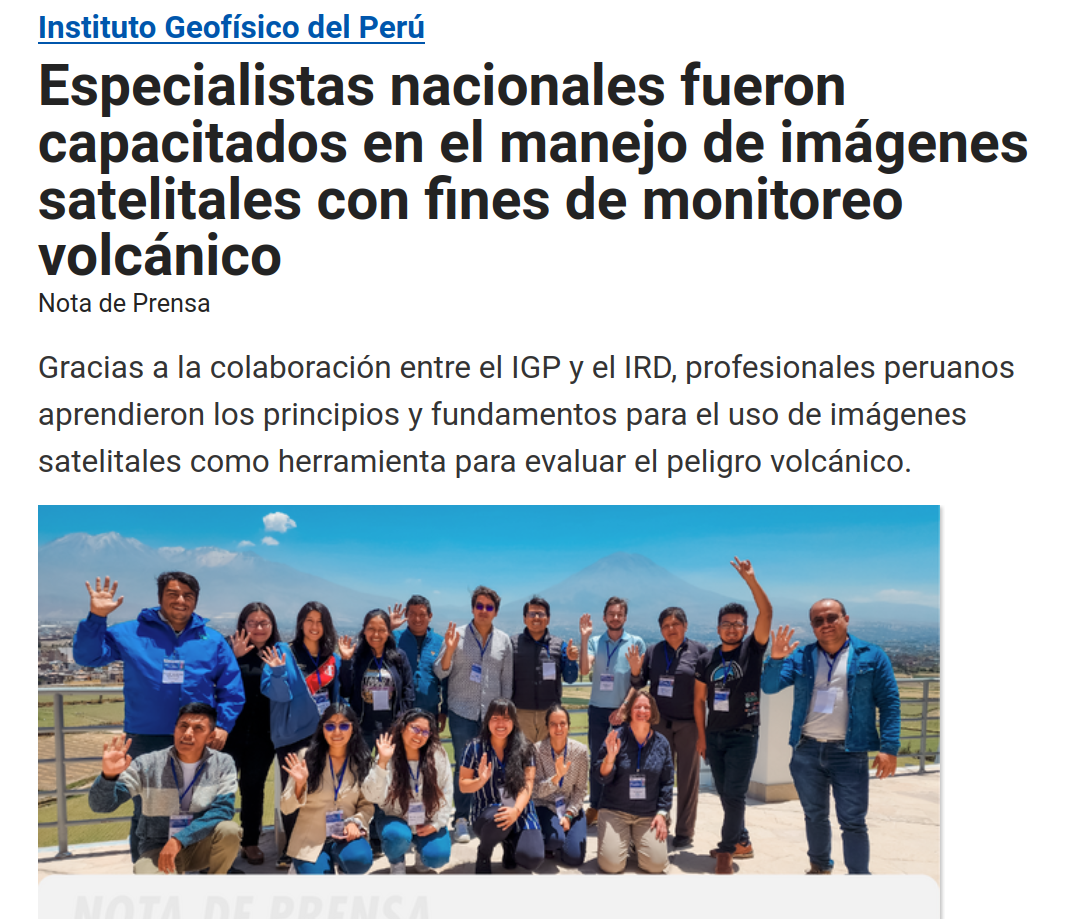
\includegraphics[width=0.9\linewidth]{images/IGP_site}
 
\end{frame}



\section{Lima}

\begin{frame}
 
 {Tasks:} \pause
 
 Template matching course 4 days from 9:30h to 16:30h \pause
 \begin{itemize}
  \item Adquisition \pause
  \item Data preparation \pause
  \item Template preparation \pause
  \item Data scanning and weighting design \pause
  \item Interpretation \pause
 \end{itemize}
 \vskip 0.5cm
 Discussions with Dr. Tavera: Masters and PhD projects. \pause
 \vskip 0.5cm
 Discussion with Dr. Norabuena: seismic and GPS data. \pause
 \vskip 0.5cm
 Discussion with Dr. Tavera: Possible new MLDs and expatriations.
 
\end{frame}


\begin{frame}

 {Template matching course}
 
 \begin{minipage}{0.45\linewidth}
  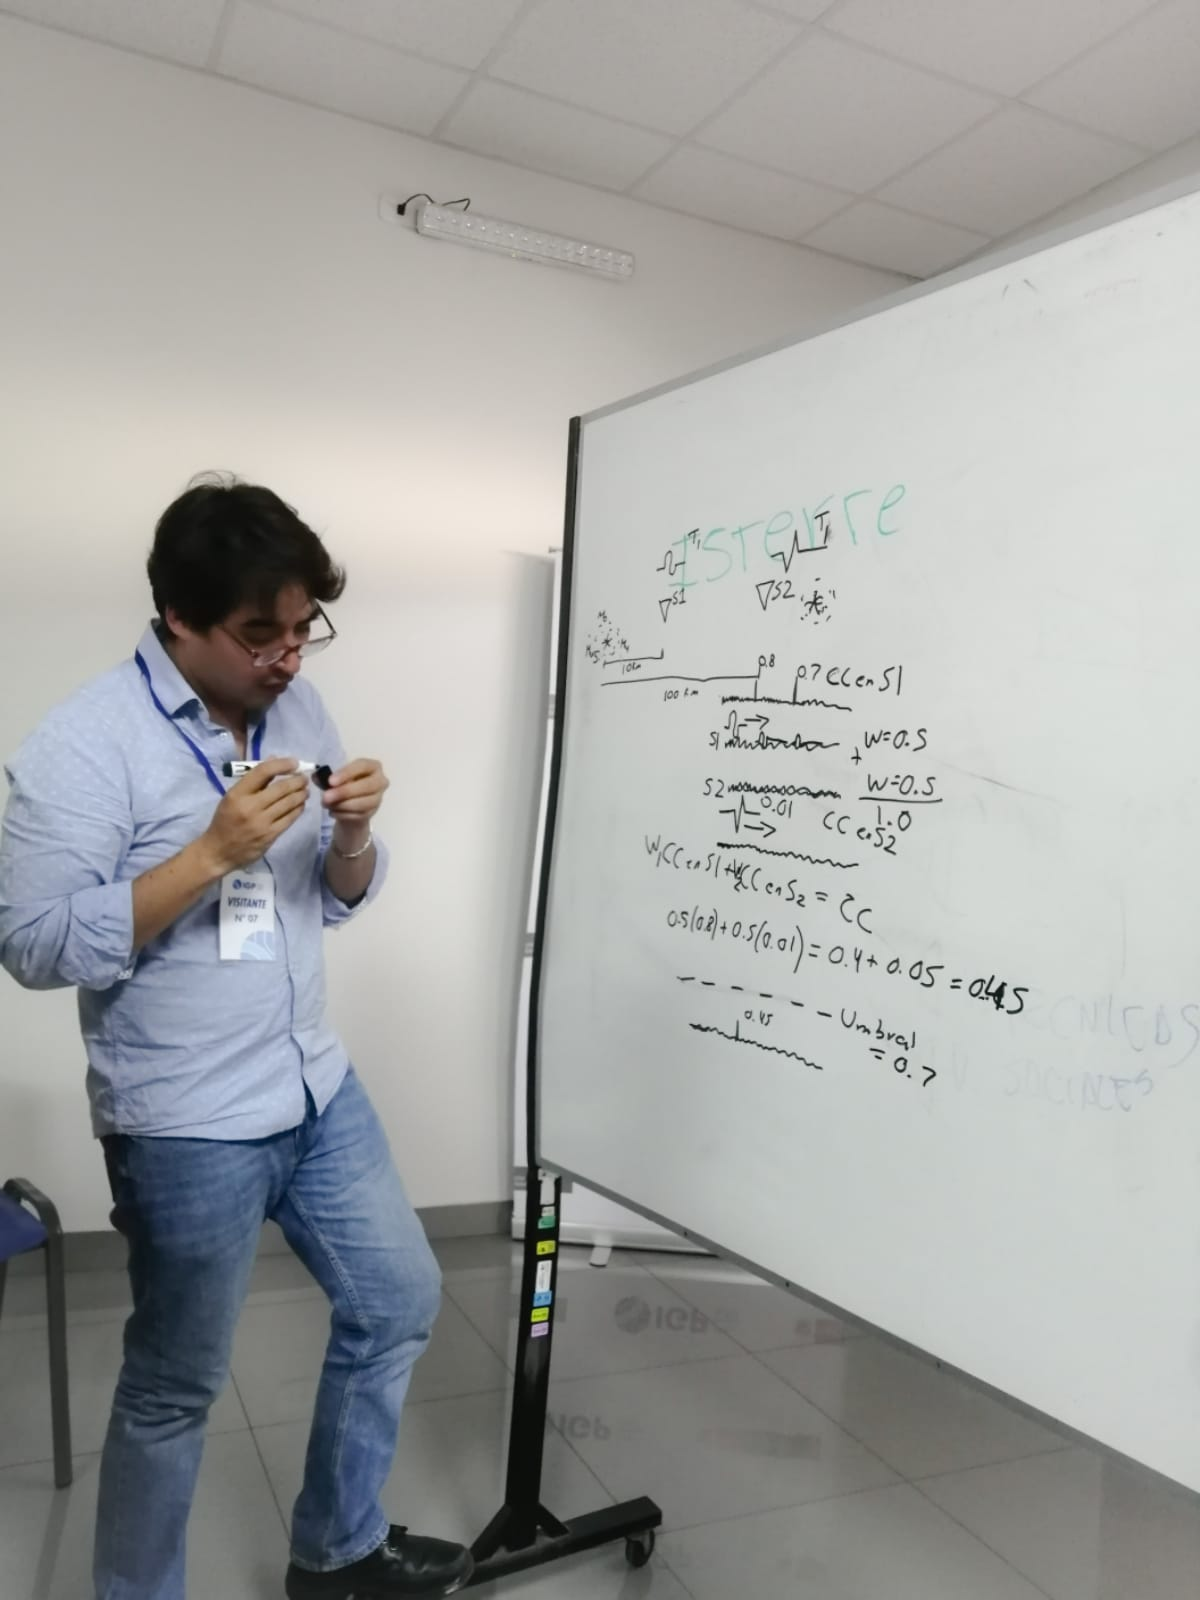
\includegraphics[width=1\linewidth]{images/Lima1}
 \end{minipage}
 \begin{minipage}{0.4\linewidth}
    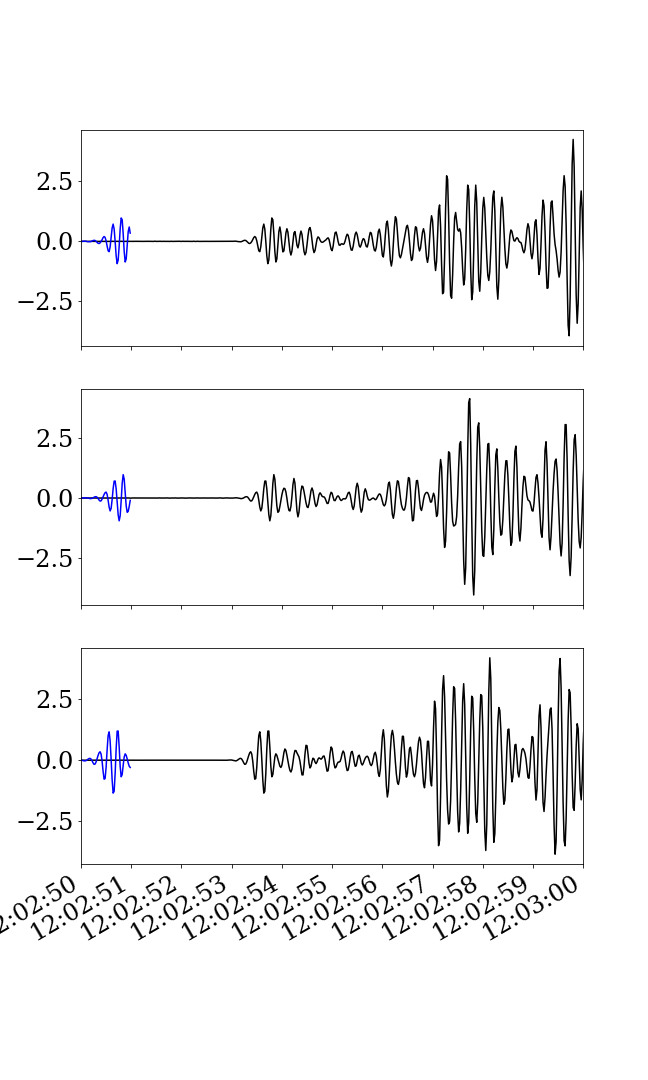
\includegraphics[width=1.2\linewidth]{images/fig_0.png}
 \end{minipage}
 
\end{frame}


\begin{frame}

 {Template matching course}
 
 \begin{minipage}{0.45\linewidth}
  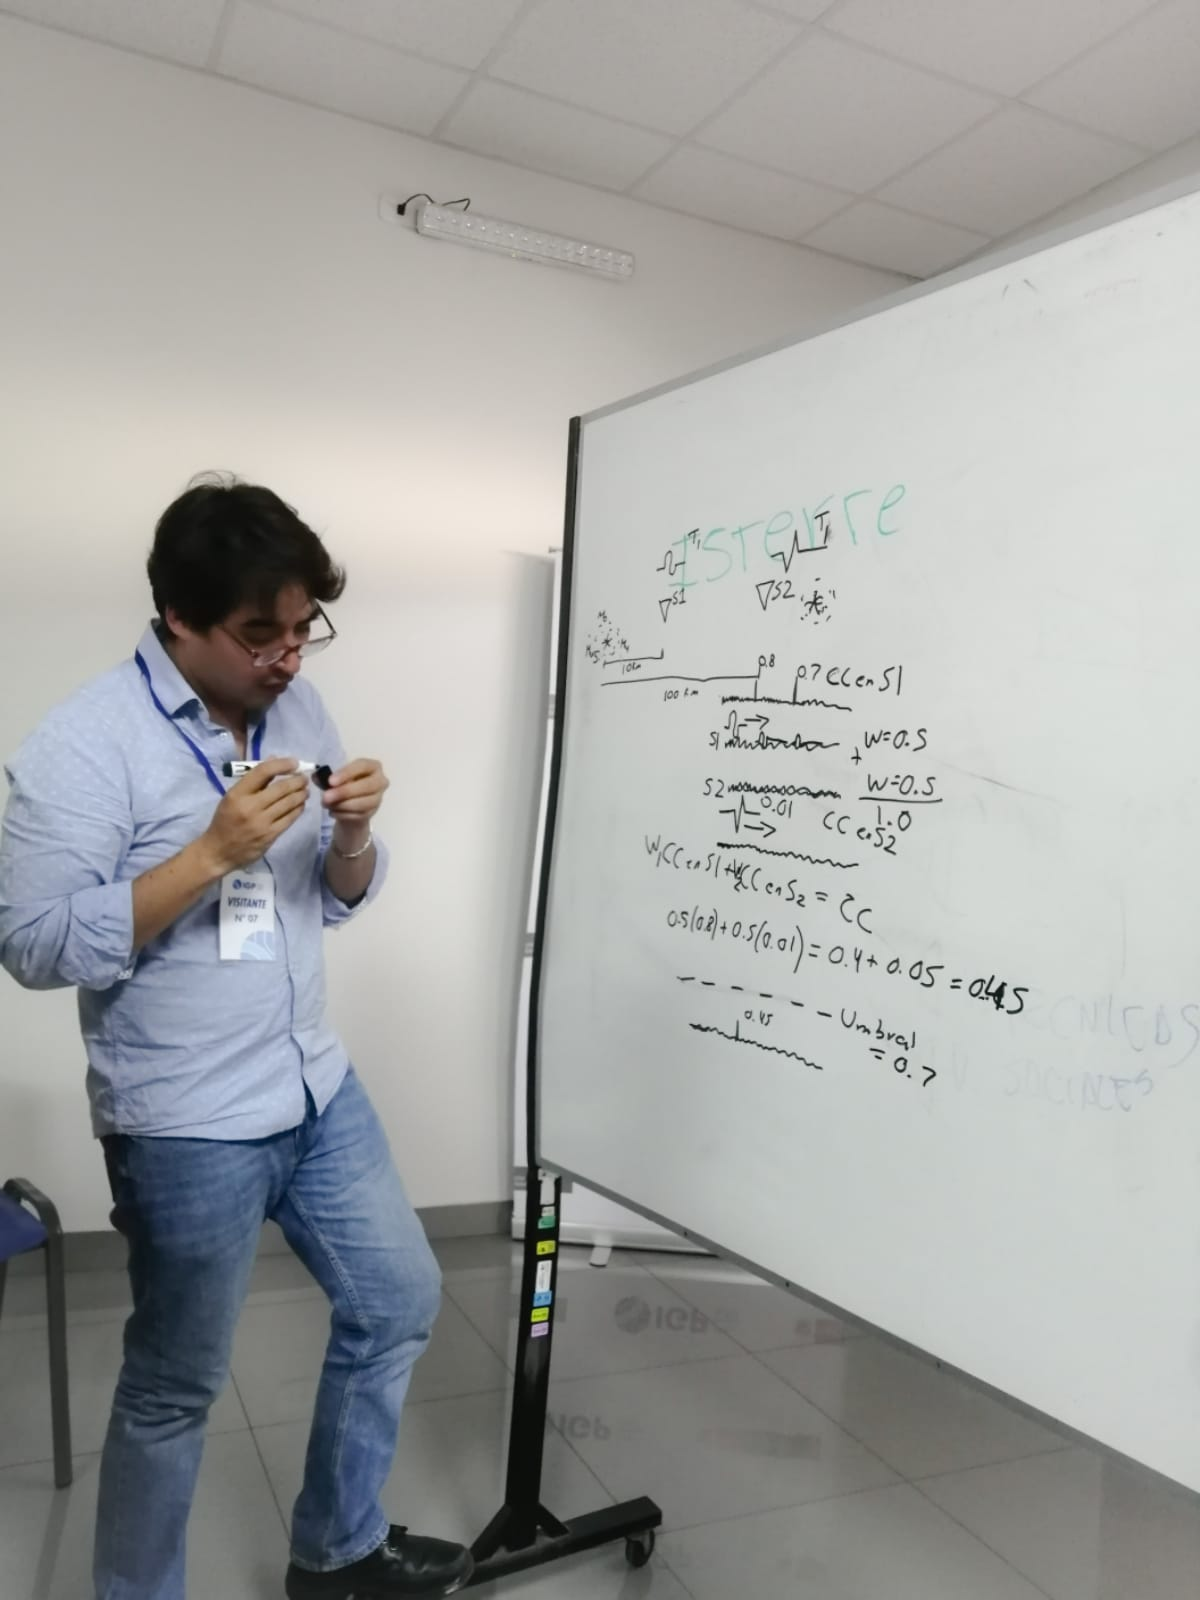
\includegraphics[width=1\linewidth]{images/Lima1}
 \end{minipage}
 \begin{minipage}{0.4\linewidth}
    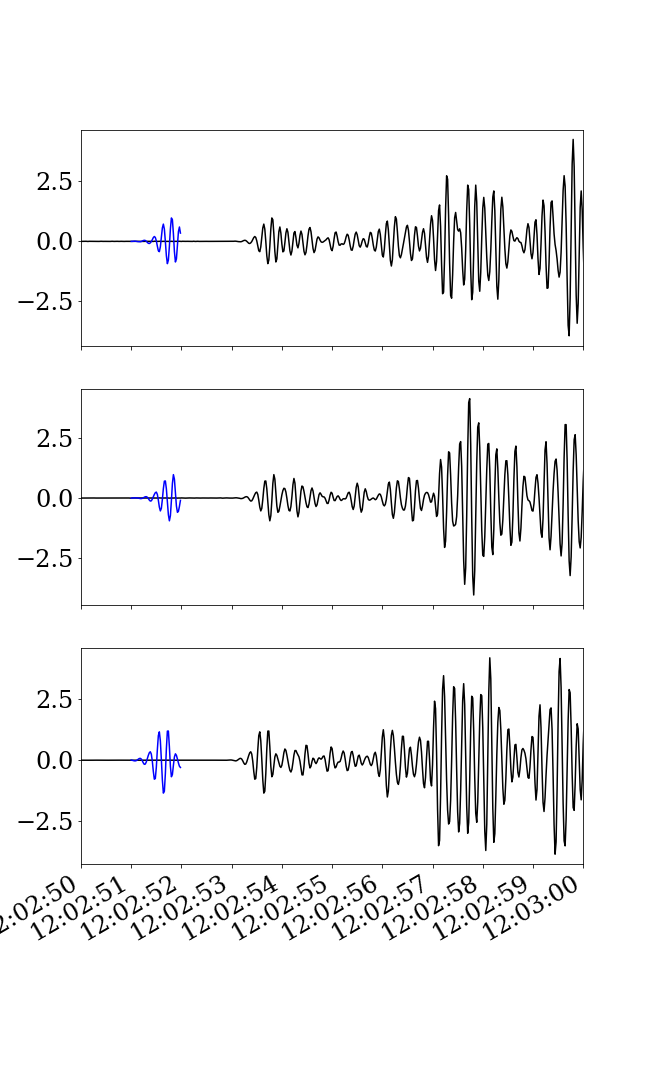
\includegraphics[width=1.2\linewidth]{images/fig_1.png}
 \end{minipage}
 
\end{frame}

\begin{frame}

 {Template matching course}
 
 \begin{minipage}{0.45\linewidth}
  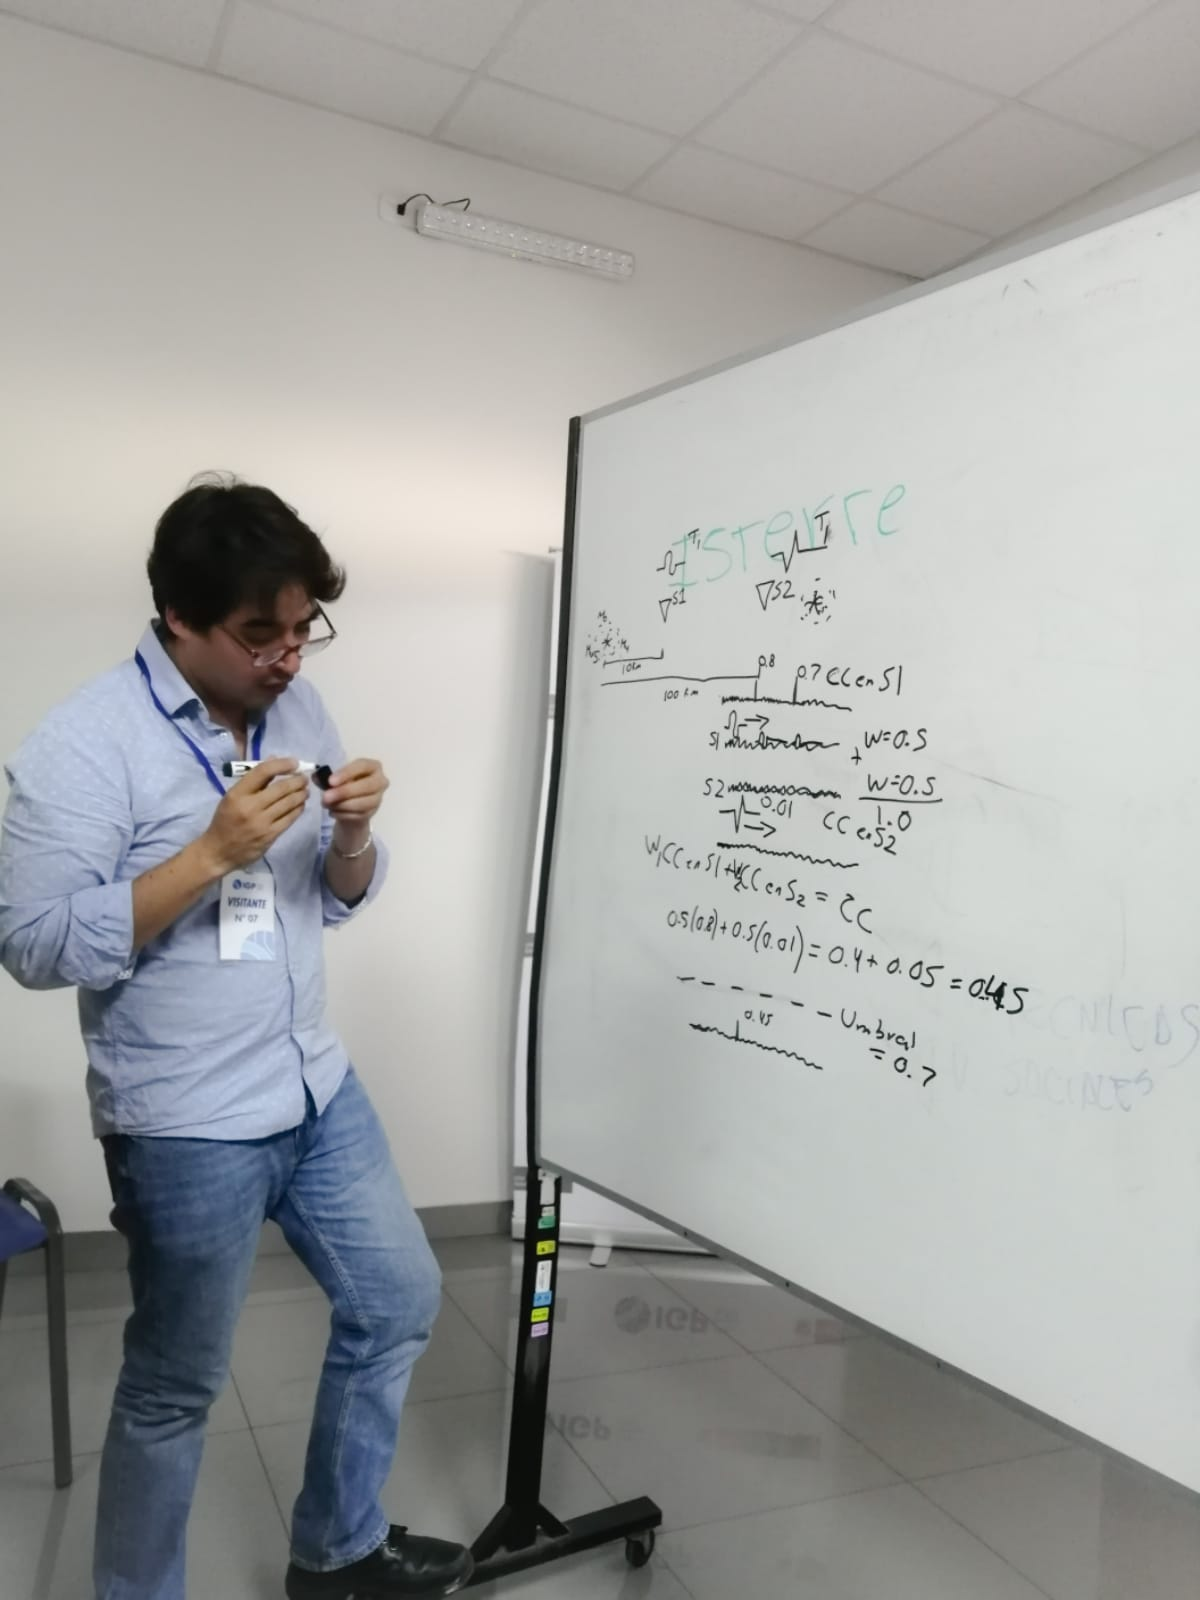
\includegraphics[width=1\linewidth]{images/Lima1}
 \end{minipage}
 \begin{minipage}{0.4\linewidth}
    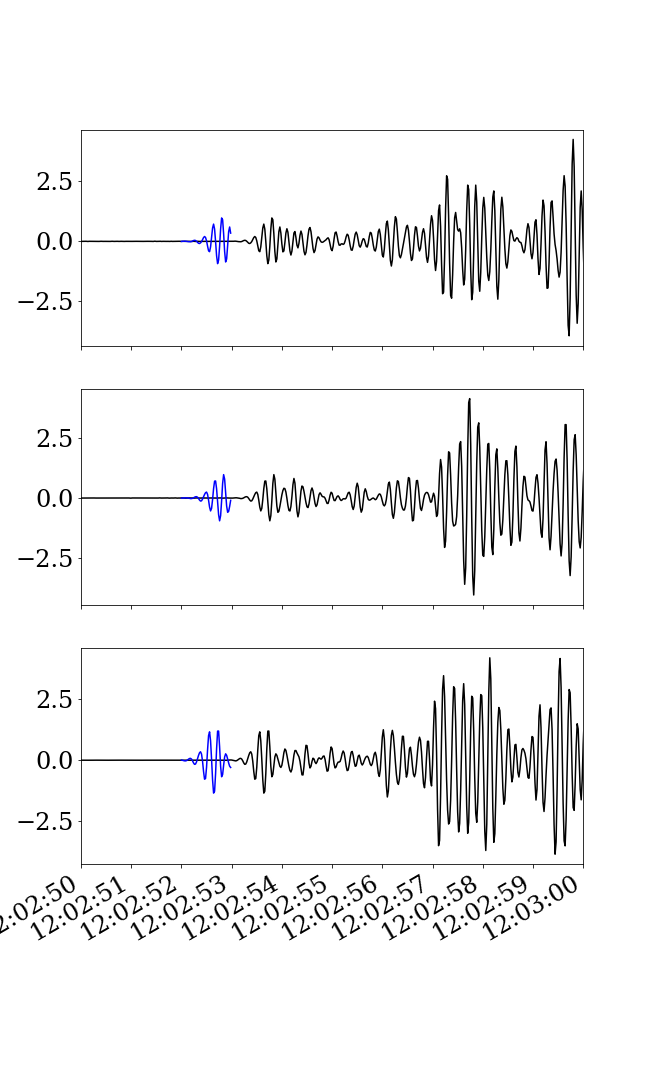
\includegraphics[width=1.2\linewidth]{images/fig_2.png}
 \end{minipage}
 
\end{frame}


\begin{frame}

 {Template matching course}
 
 \begin{minipage}{0.45\linewidth}
  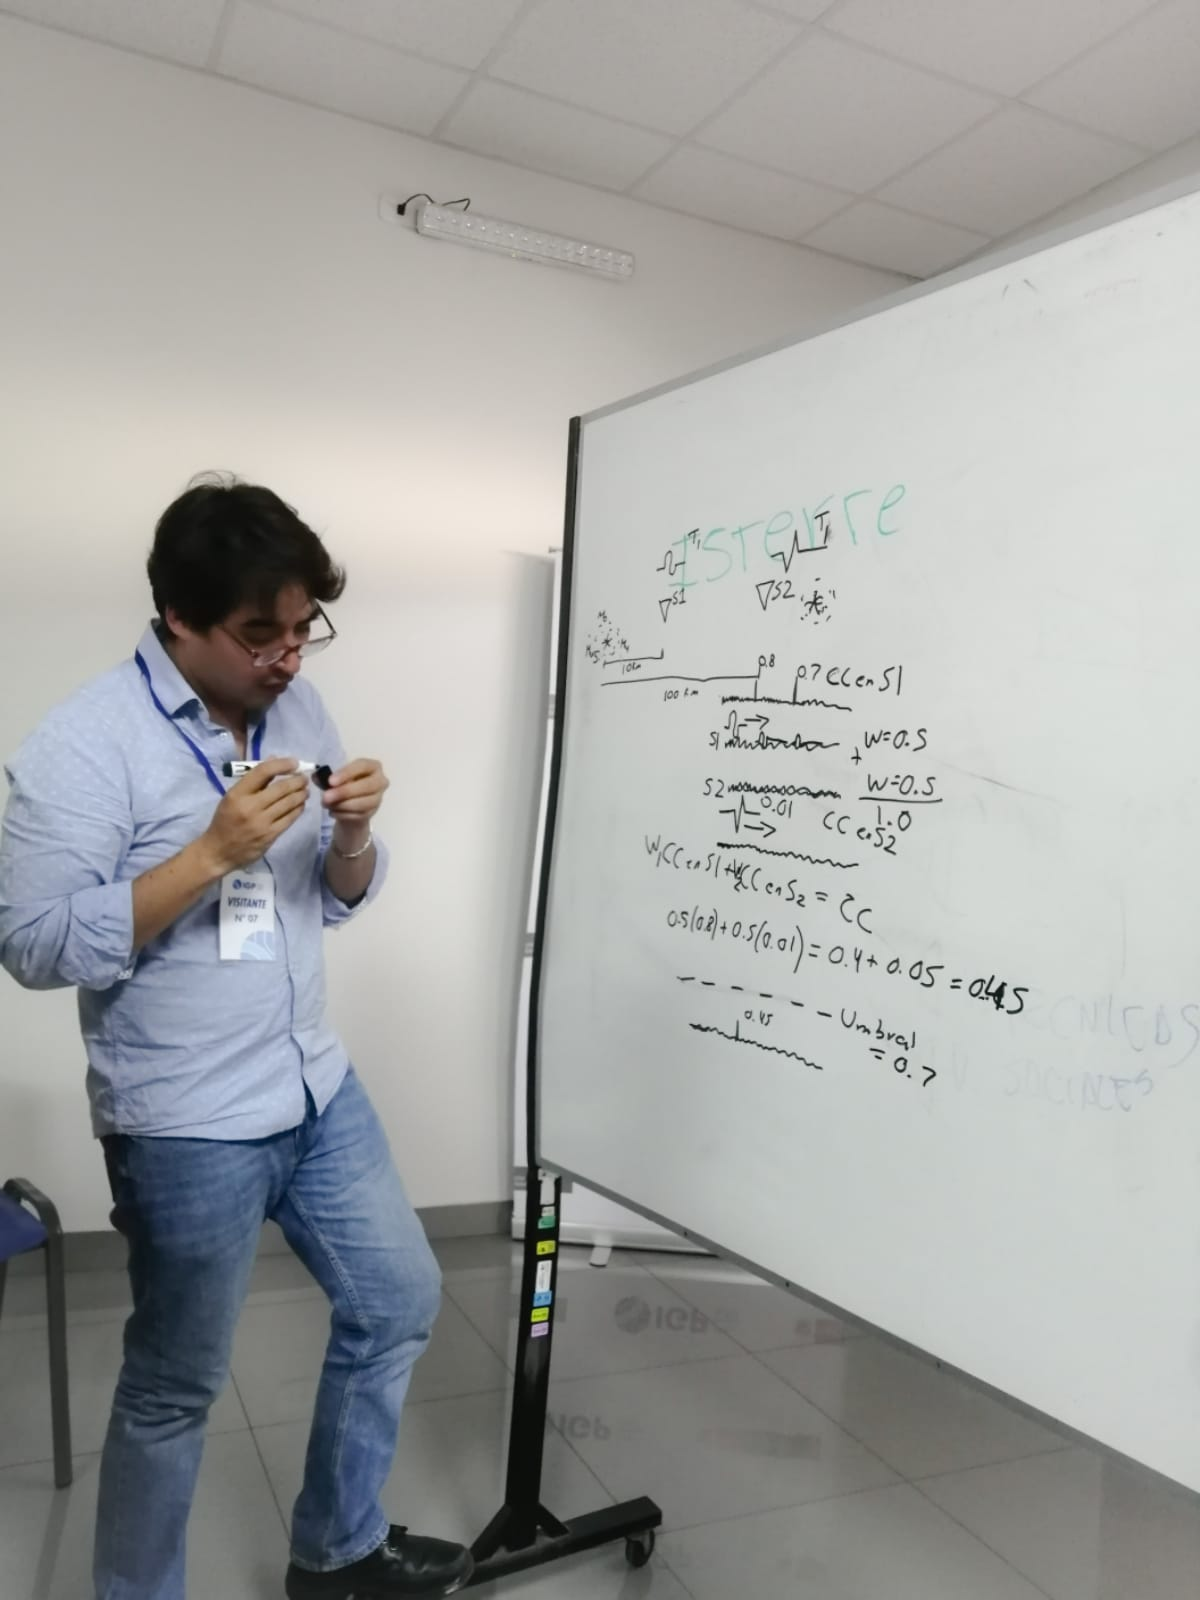
\includegraphics[width=1\linewidth]{images/Lima1}
 \end{minipage}
 \begin{minipage}{0.4\linewidth}
    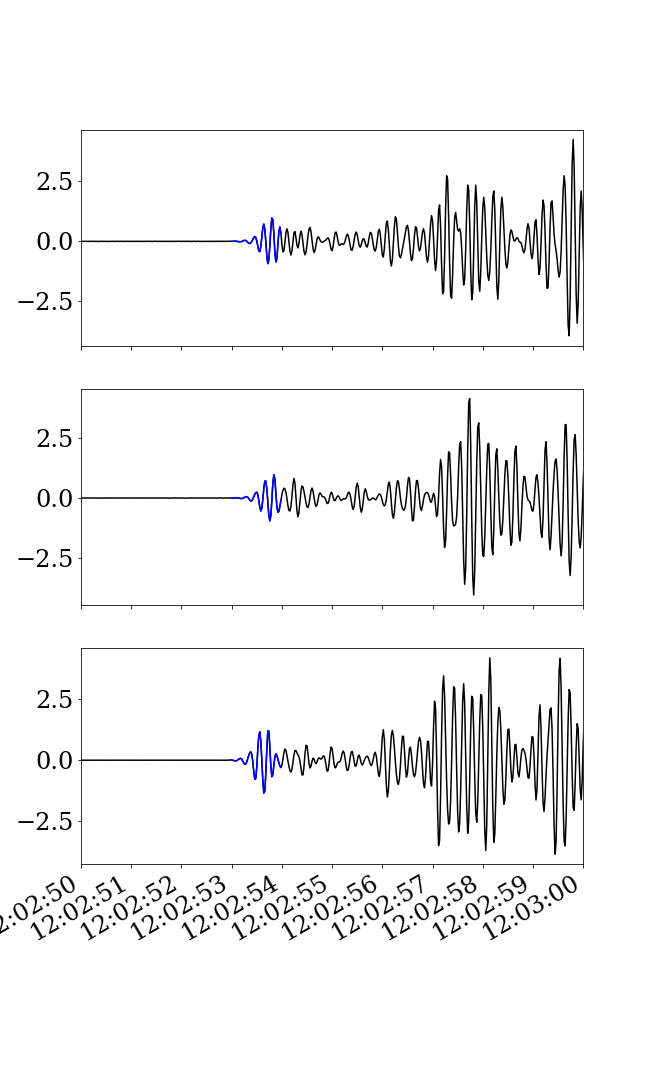
\includegraphics[width=1.2\linewidth]{images/fig_3.png}
 \end{minipage}
 
\end{frame}


\begin{frame}

 {Template matching course}
 
 \begin{minipage}{0.45\linewidth}
  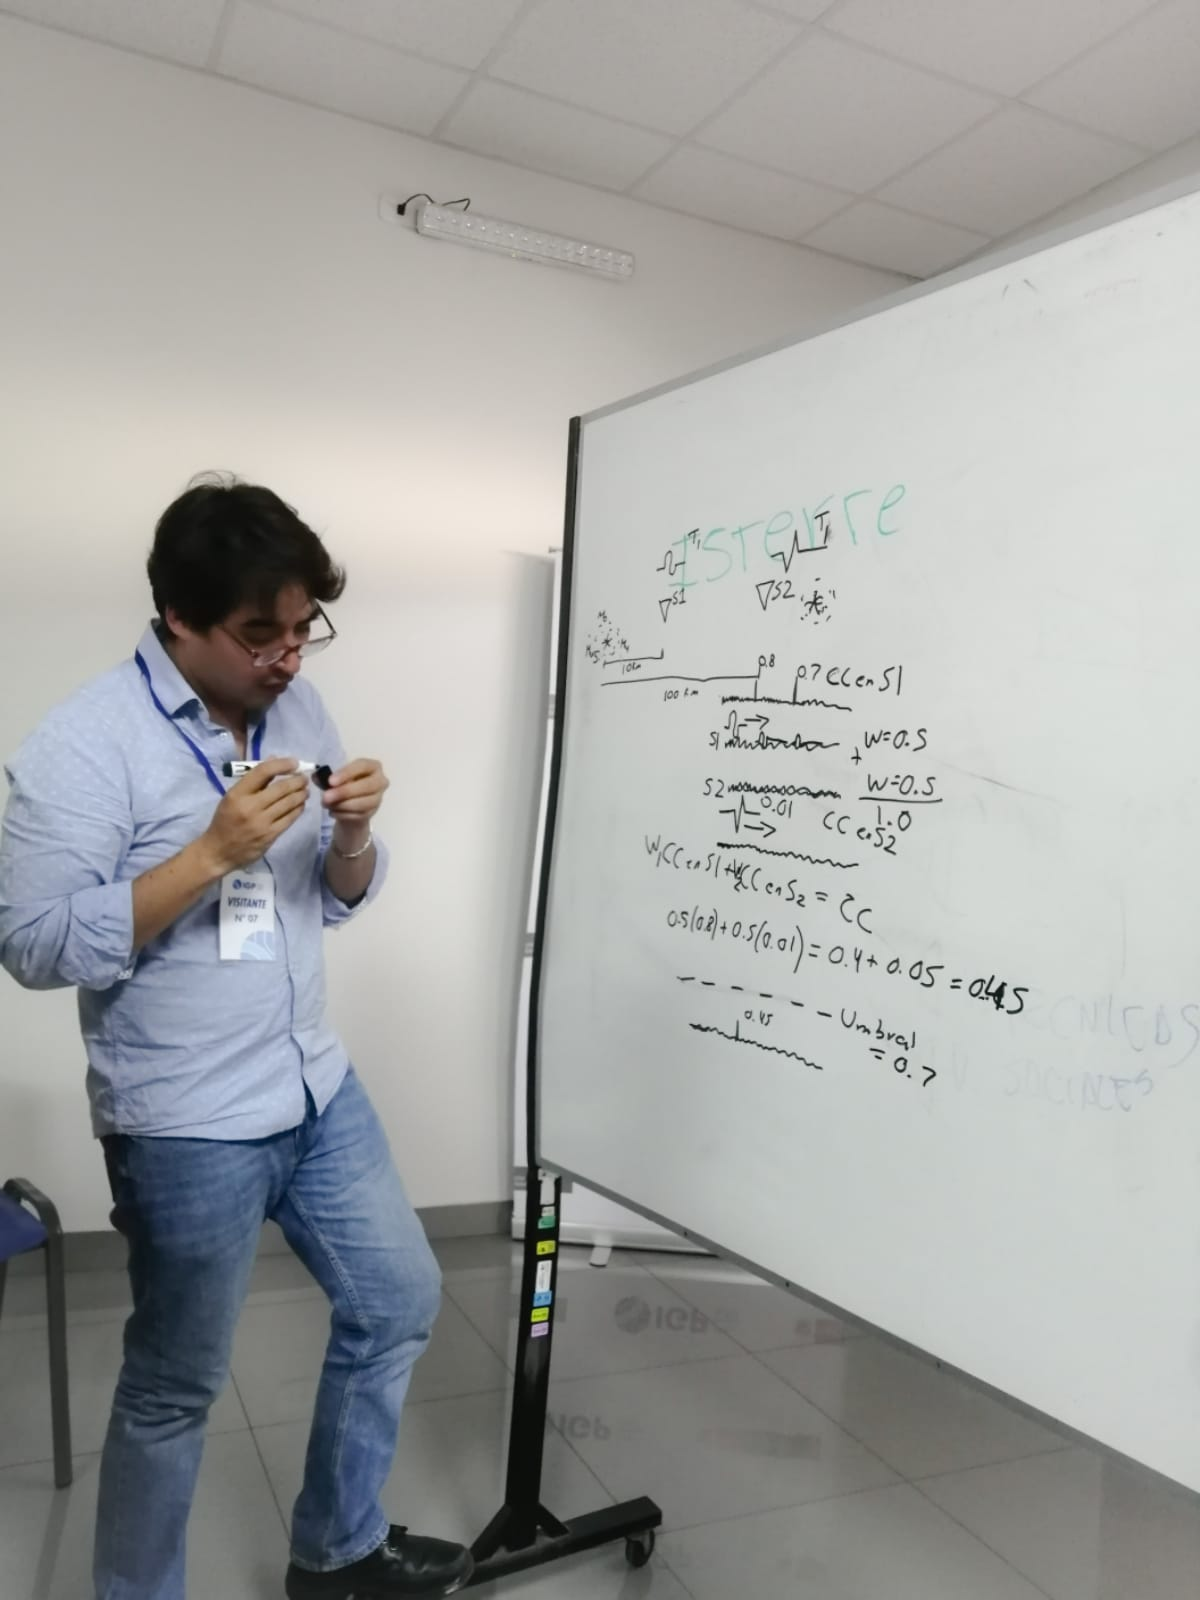
\includegraphics[width=1\linewidth]{images/Lima1}
 \end{minipage}
 \begin{minipage}{0.4\linewidth}
    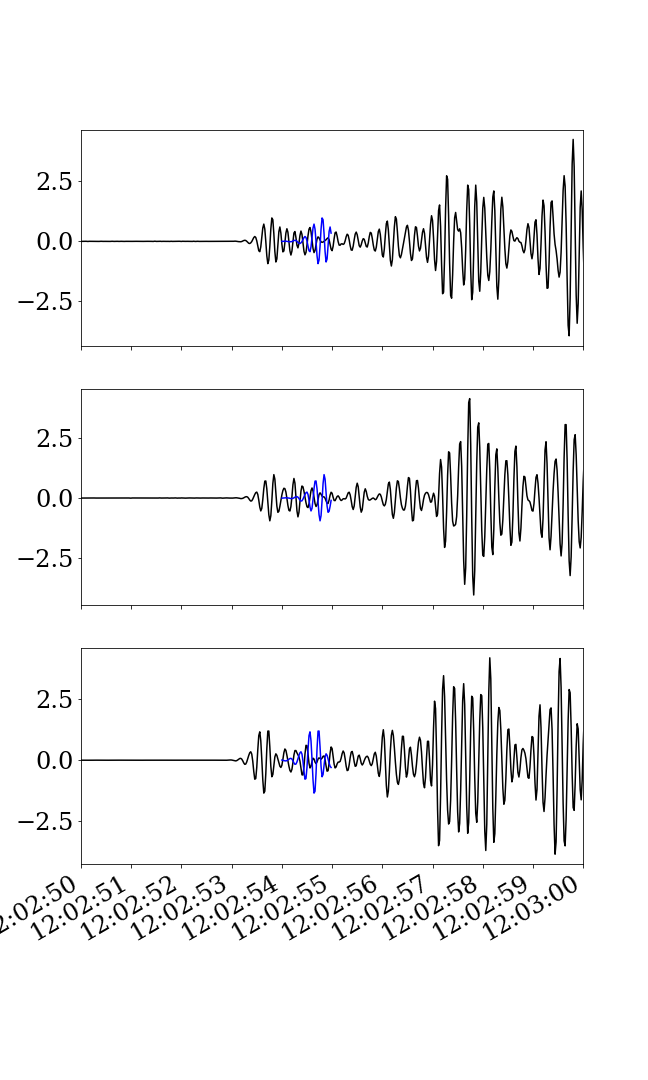
\includegraphics[width=1.2\linewidth]{images/fig_4.png}
 \end{minipage}
 
\end{frame}


\begin{frame}

 {Template matching course}
 
 \begin{minipage}{0.45\linewidth}
  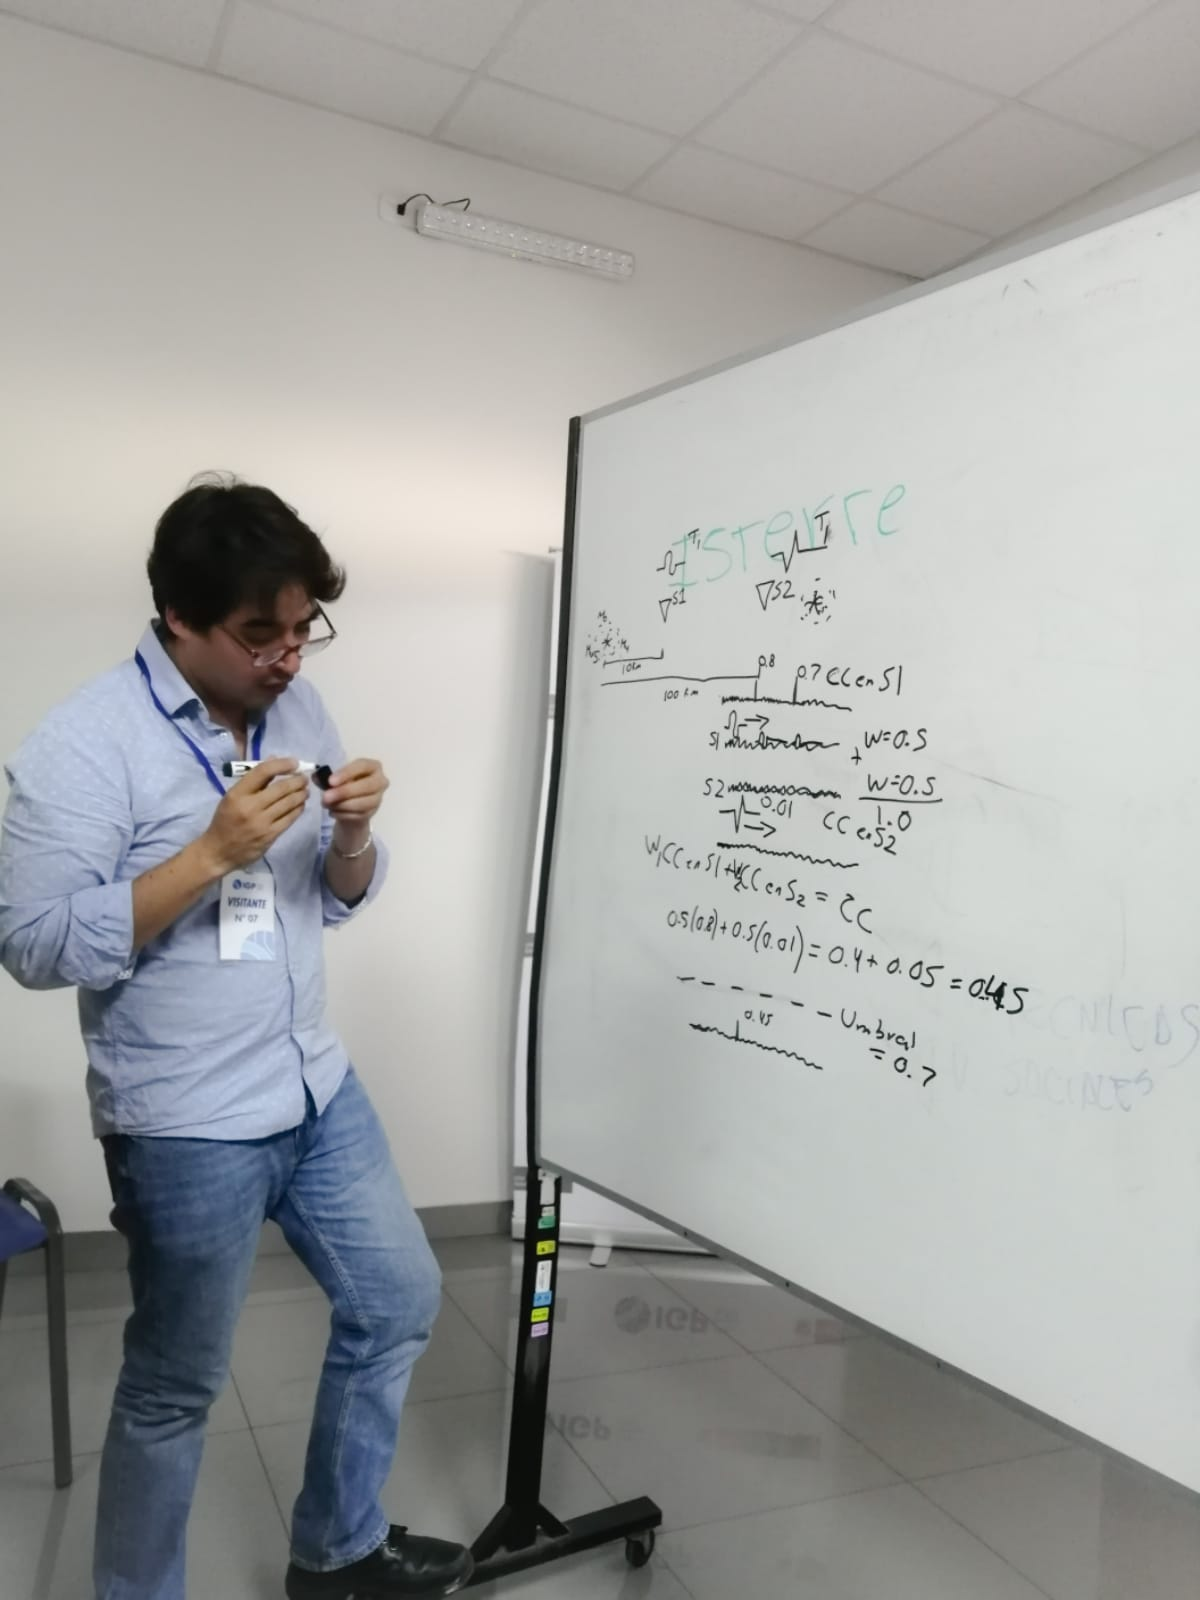
\includegraphics[width=1\linewidth]{images/Lima1}
 \end{minipage}
 \begin{minipage}{0.4\linewidth}
    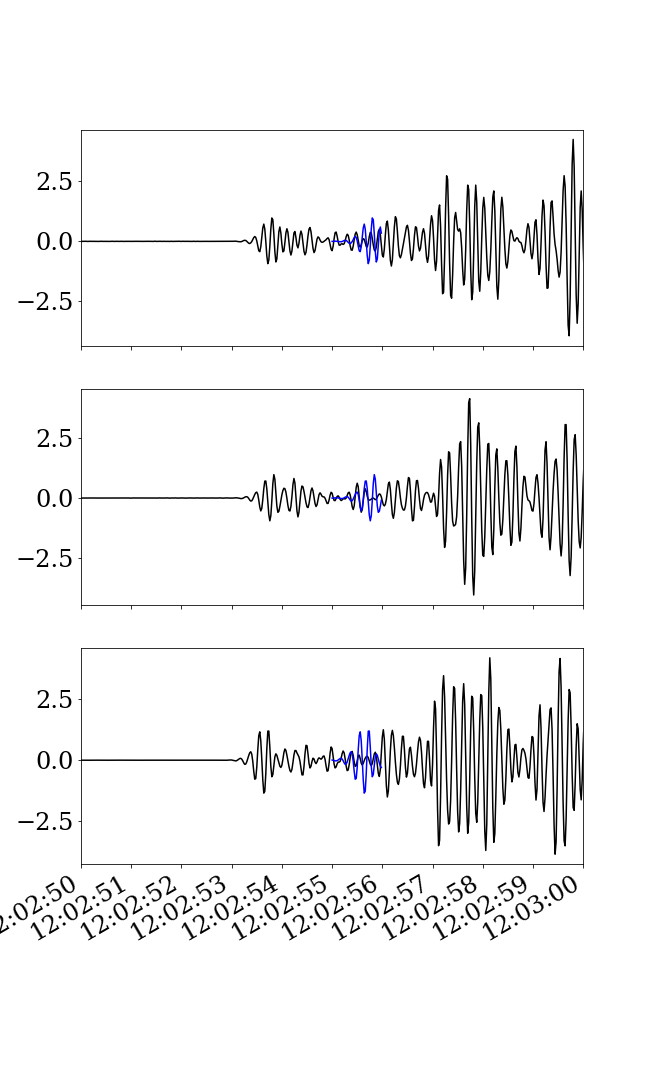
\includegraphics[width=1.2\linewidth]{images/fig_5.png}
 \end{minipage}
 
\end{frame}


\begin{frame}

 {Template matching course}
 
 \begin{minipage}{0.45\linewidth}
  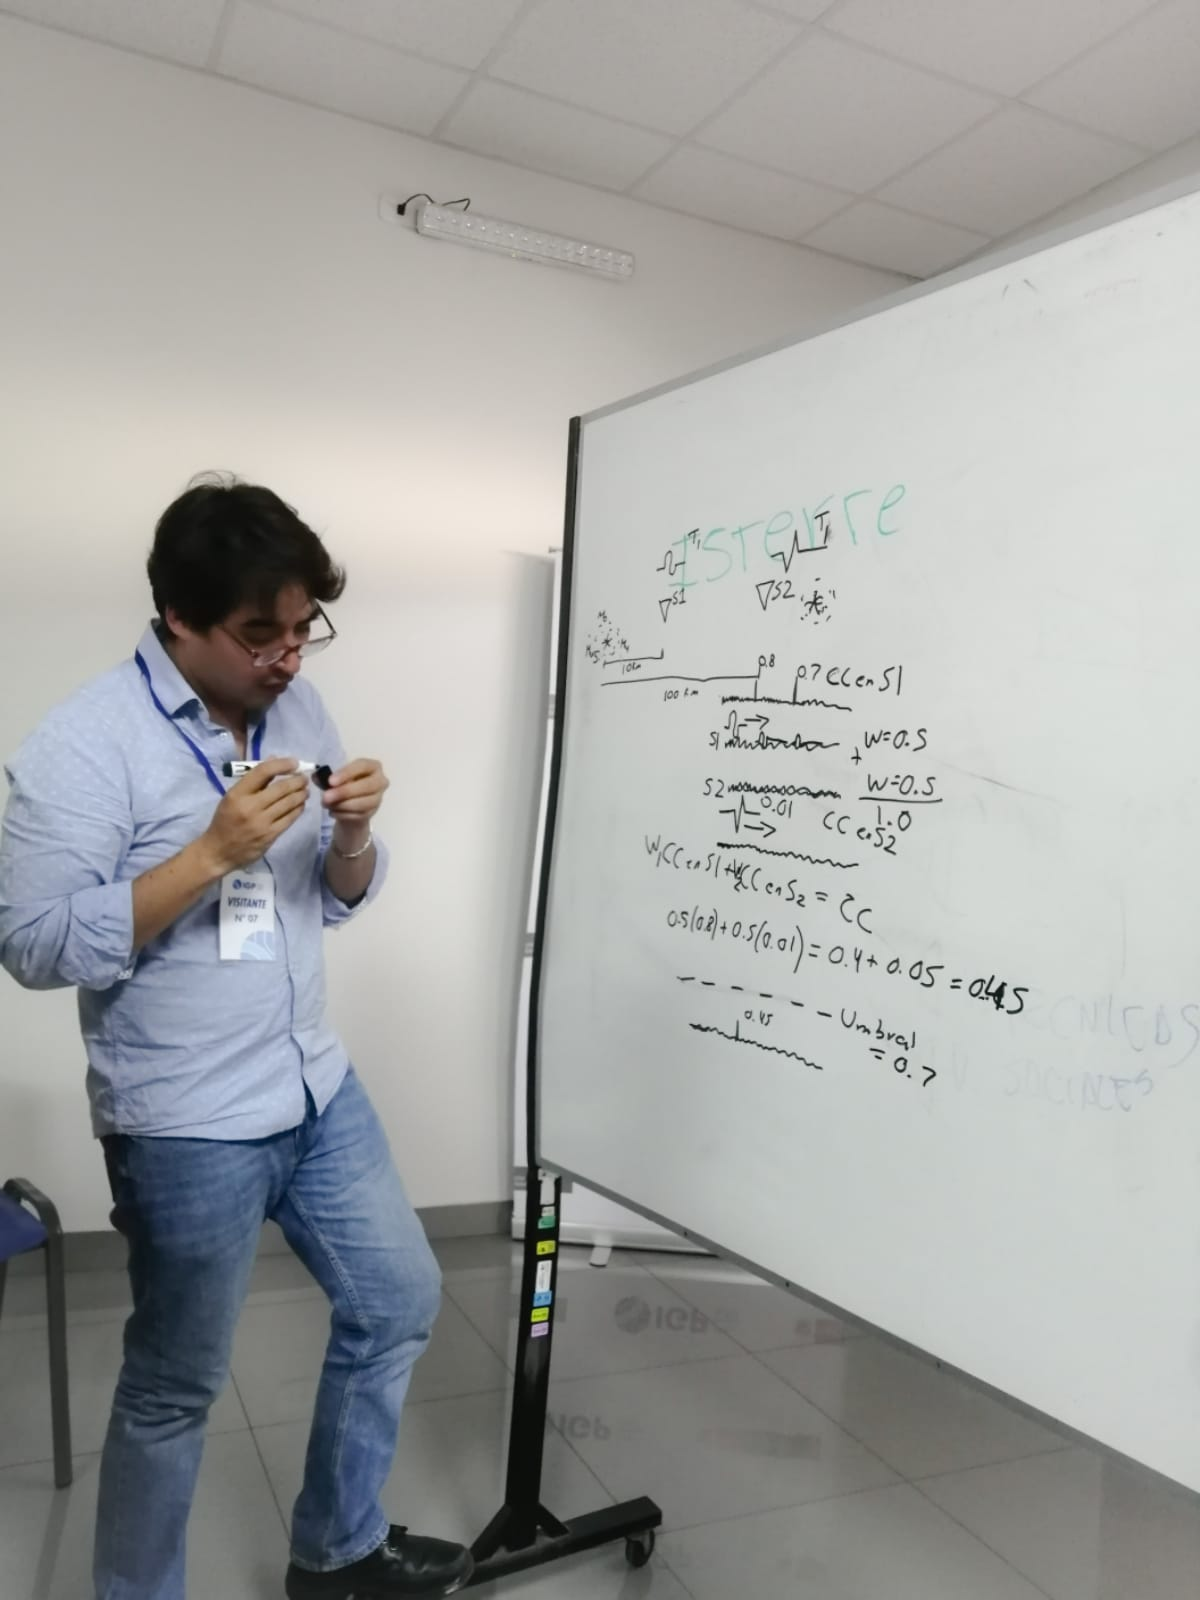
\includegraphics[width=1\linewidth]{images/Lima1}
 \end{minipage}
 \begin{minipage}{0.4\linewidth}
    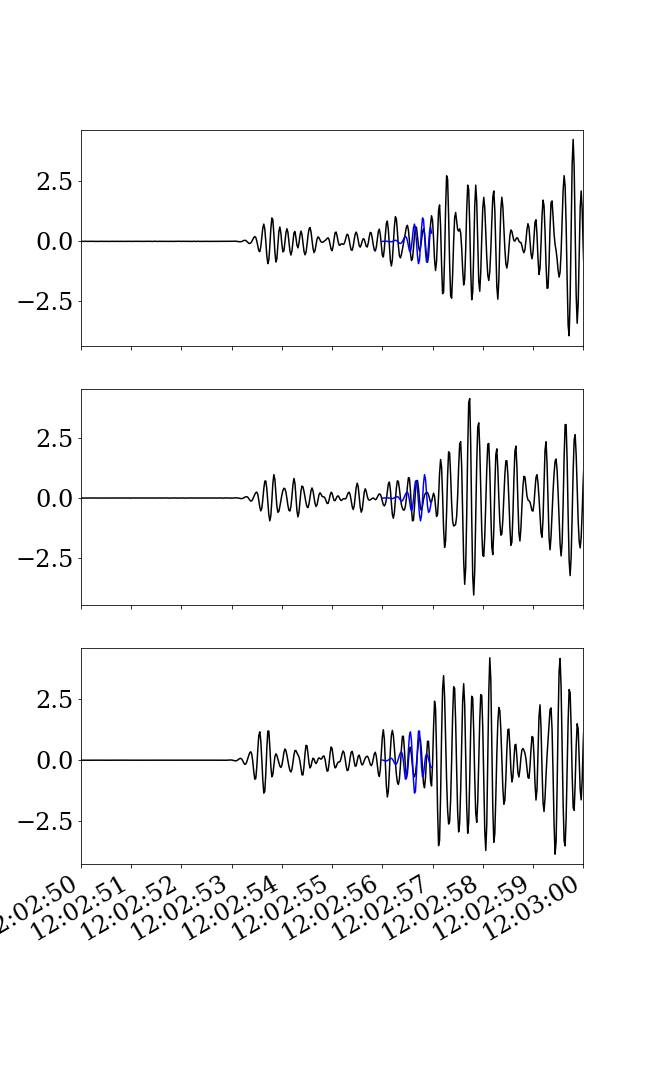
\includegraphics[width=1.2\linewidth]{images/fig_6.png}
 \end{minipage}
 
\end{frame}

\begin{frame}
 
 {During the course: IGP Lima}
 
 \begin{minipage}{0.45\linewidth}
   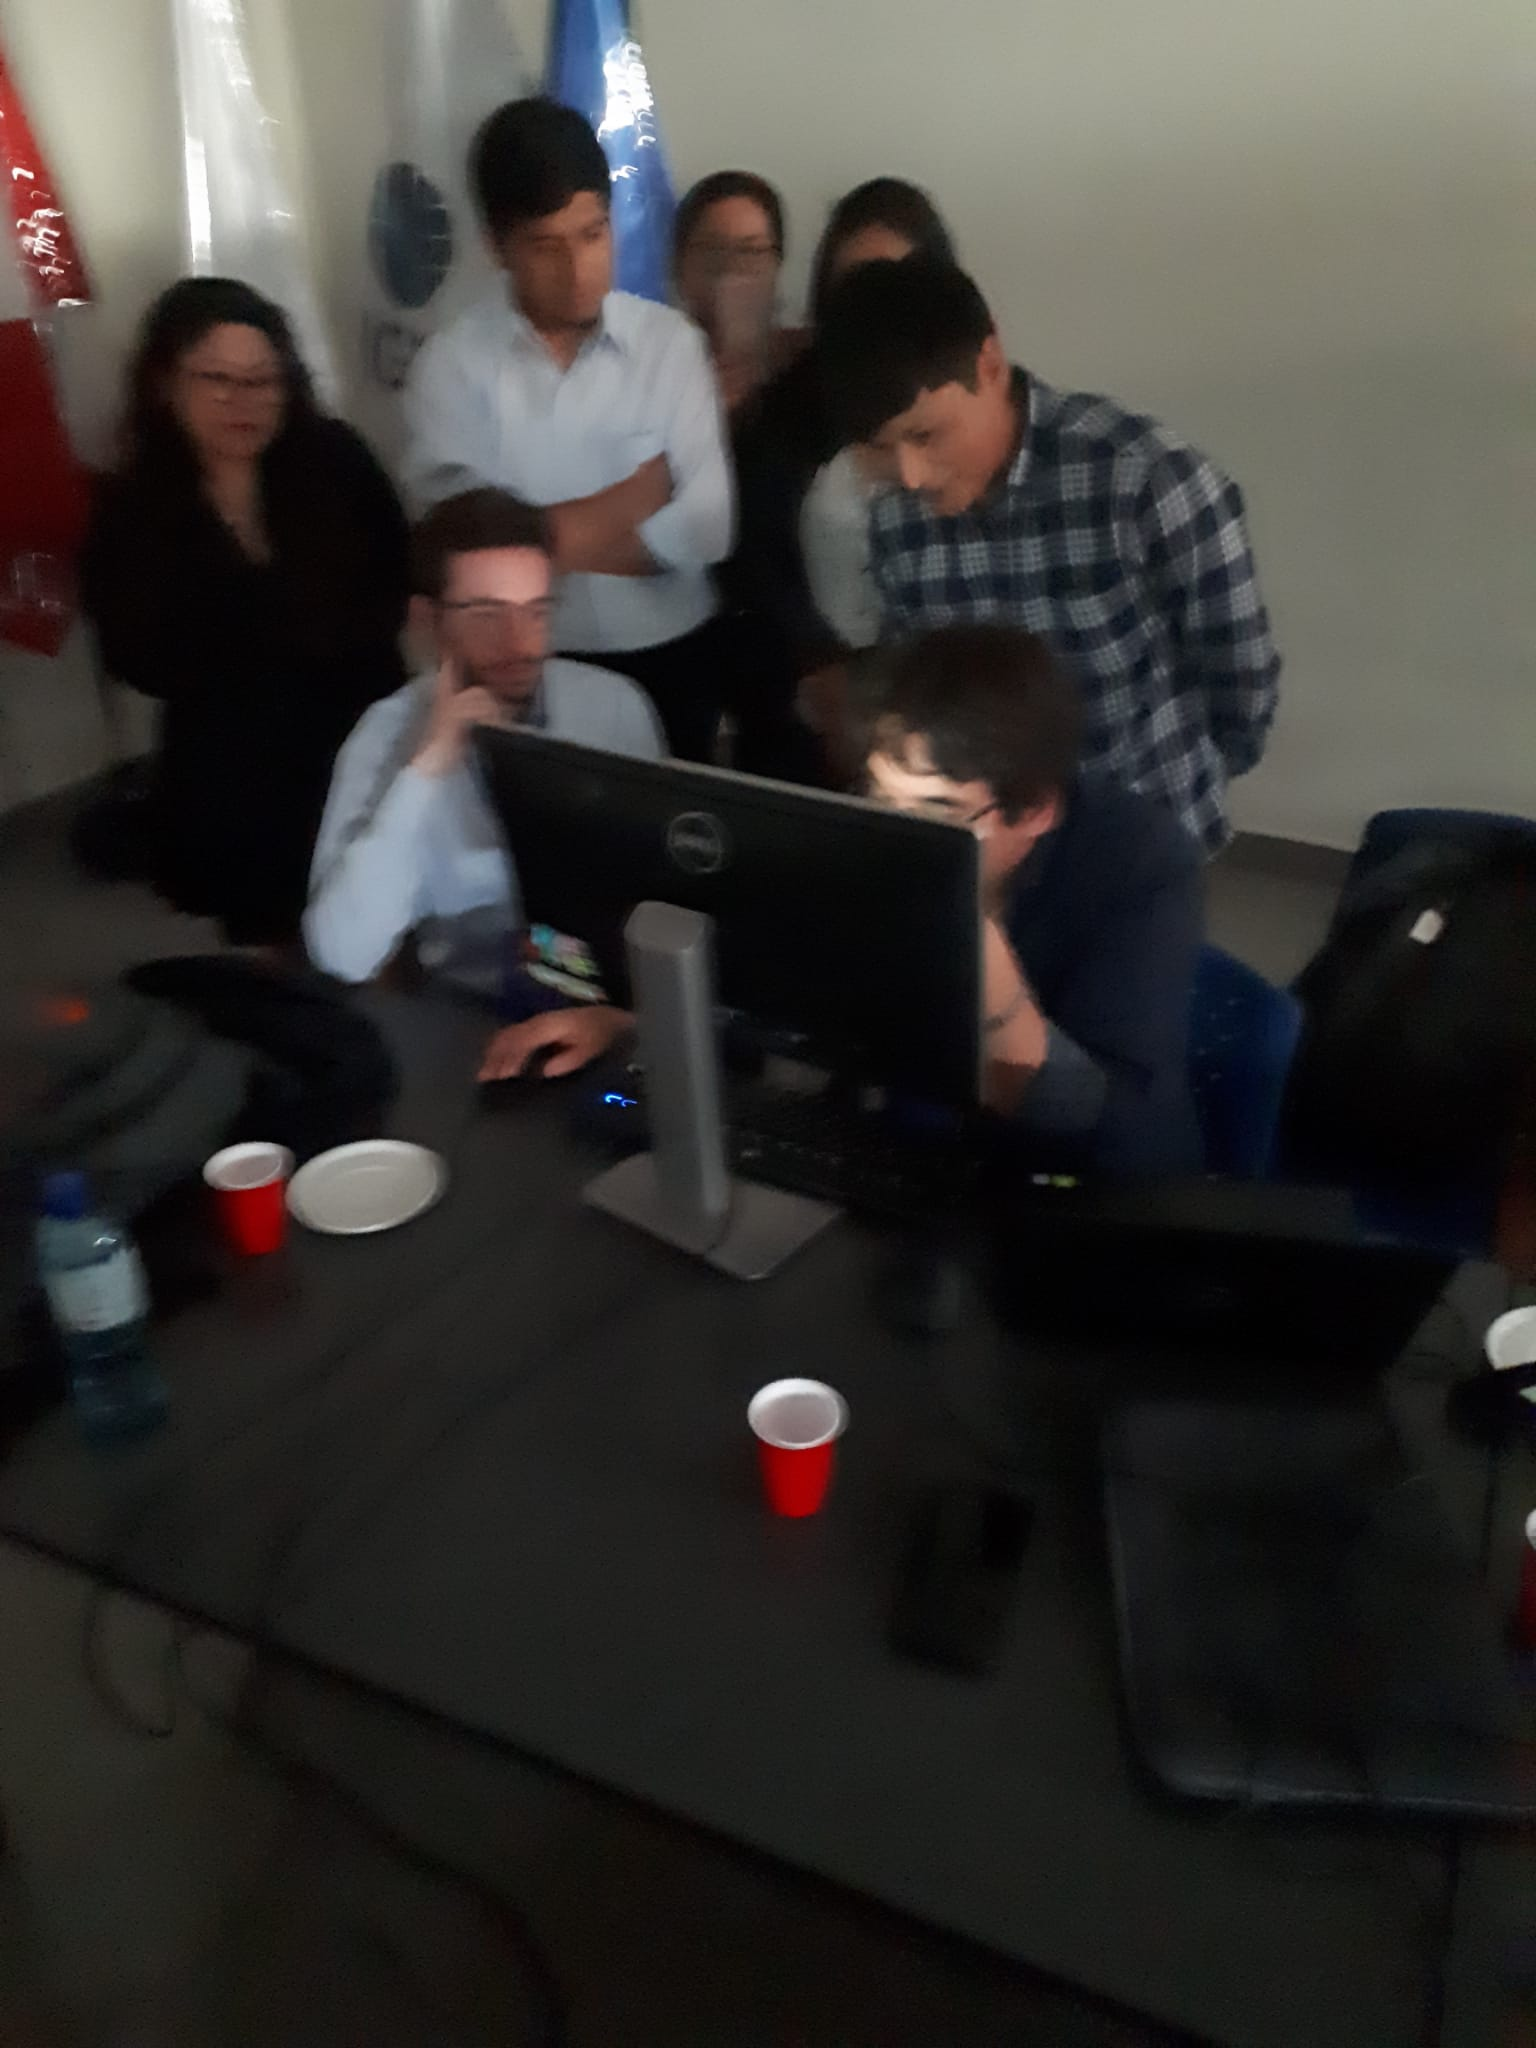
\includegraphics[width=1\linewidth]{images/Lima2}
 \end{minipage}
 \begin{minipage}{0.45\linewidth}
   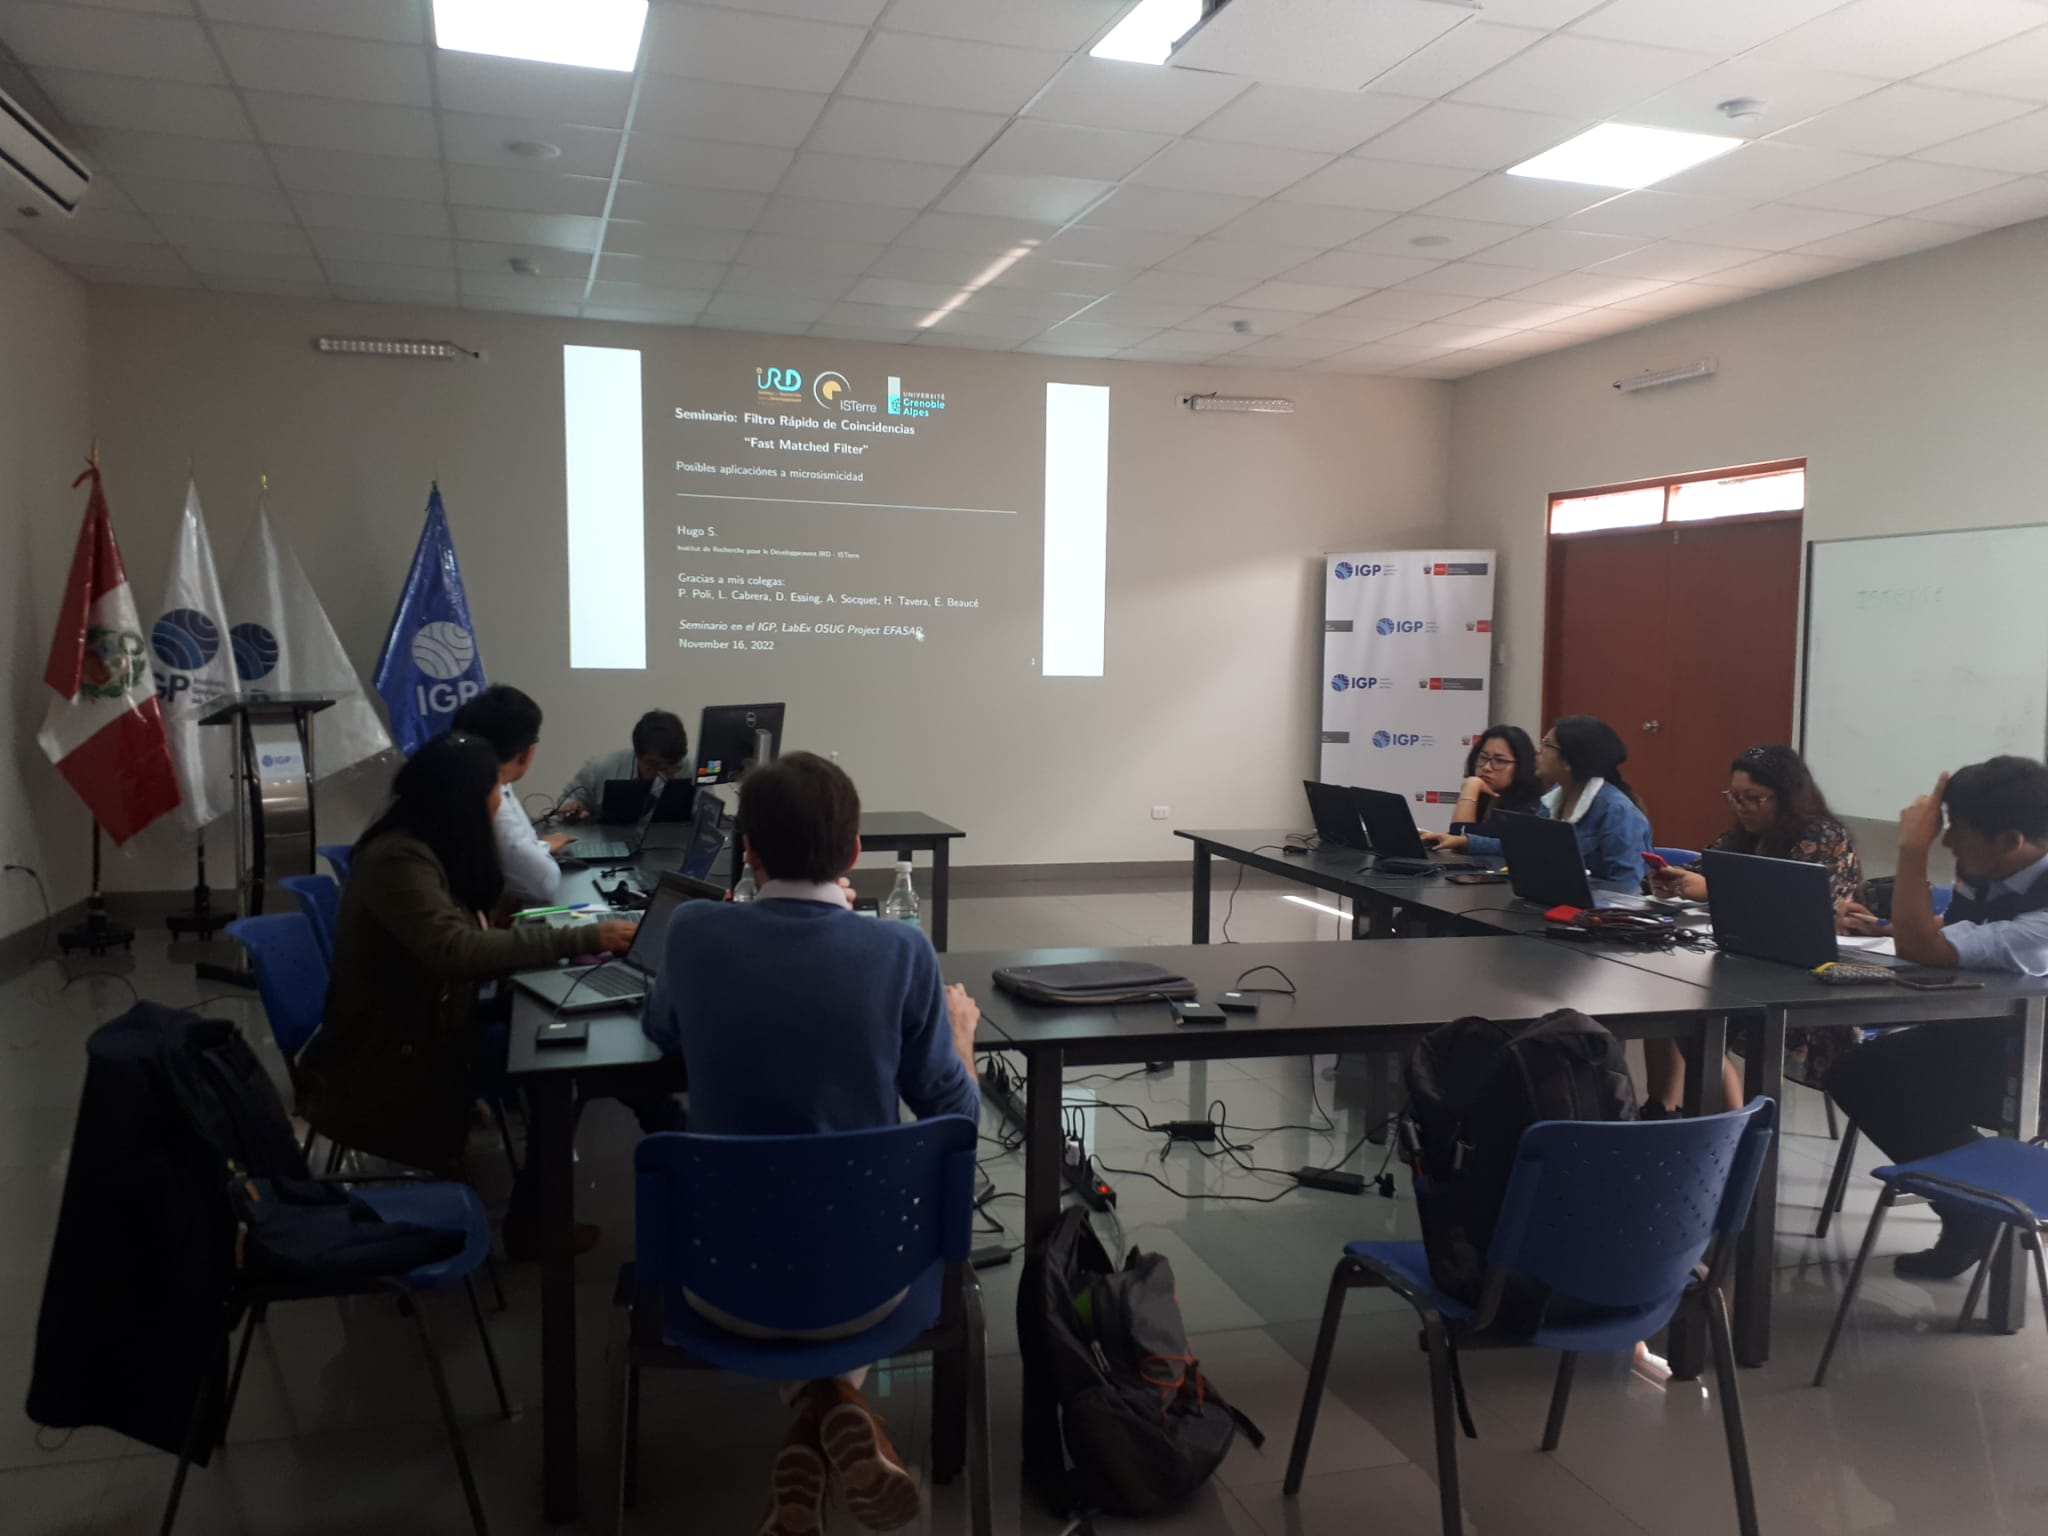
\includegraphics[width=1\linewidth]{images/Lima3}
 \end{minipage}

 
\end{frame}



\begin{frame}
 
 {Mission completed!}
 
 \begin{minipage}{0.45\linewidth}
  \vskip 1cm
   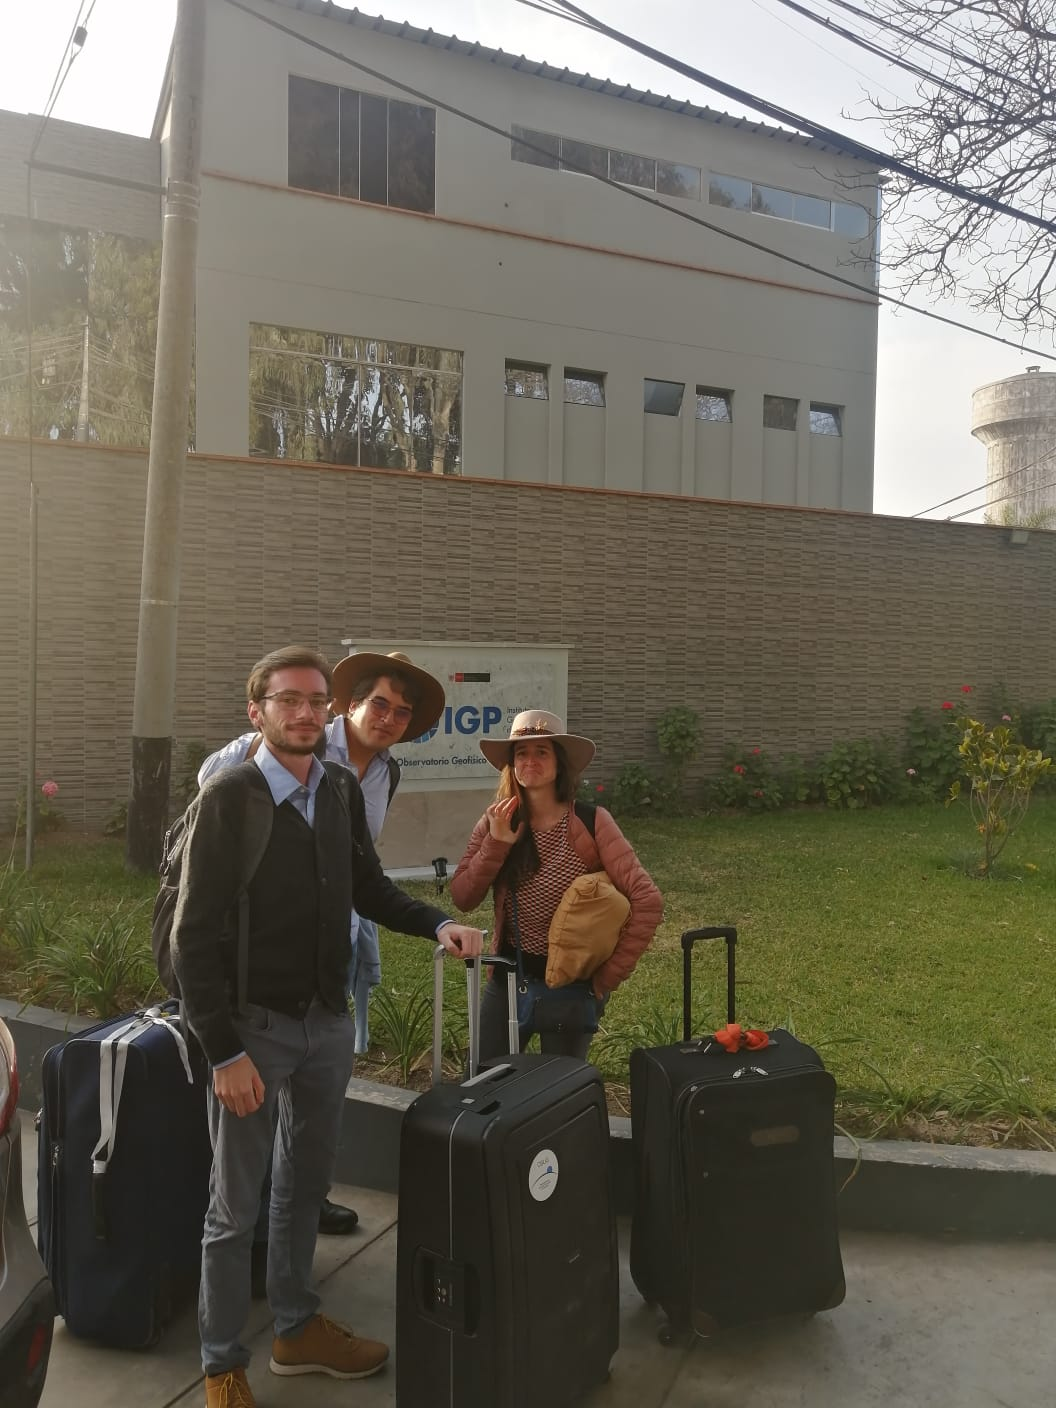
\includegraphics[width=1\linewidth]{images/Lima5}
 \end{minipage}
 \begin{minipage}{0.45\linewidth}
 Thank you very much to:
  \begin{itemize}
   \item Virginie Pinel
   \item L\'ea Pousse
   \item Bertrand Lovery
   \item Hernando Tavera
   \item IGP Staff: Estela, Arturo, Vilma, Juan Carlos, Katy, Christian, Paco
  \end{itemize}

 
 \end{minipage}

 
\end{frame}



\section{PhD. Project ARTS}

\begin{frame}
 
 {Local network: Valle del Colca}
 
 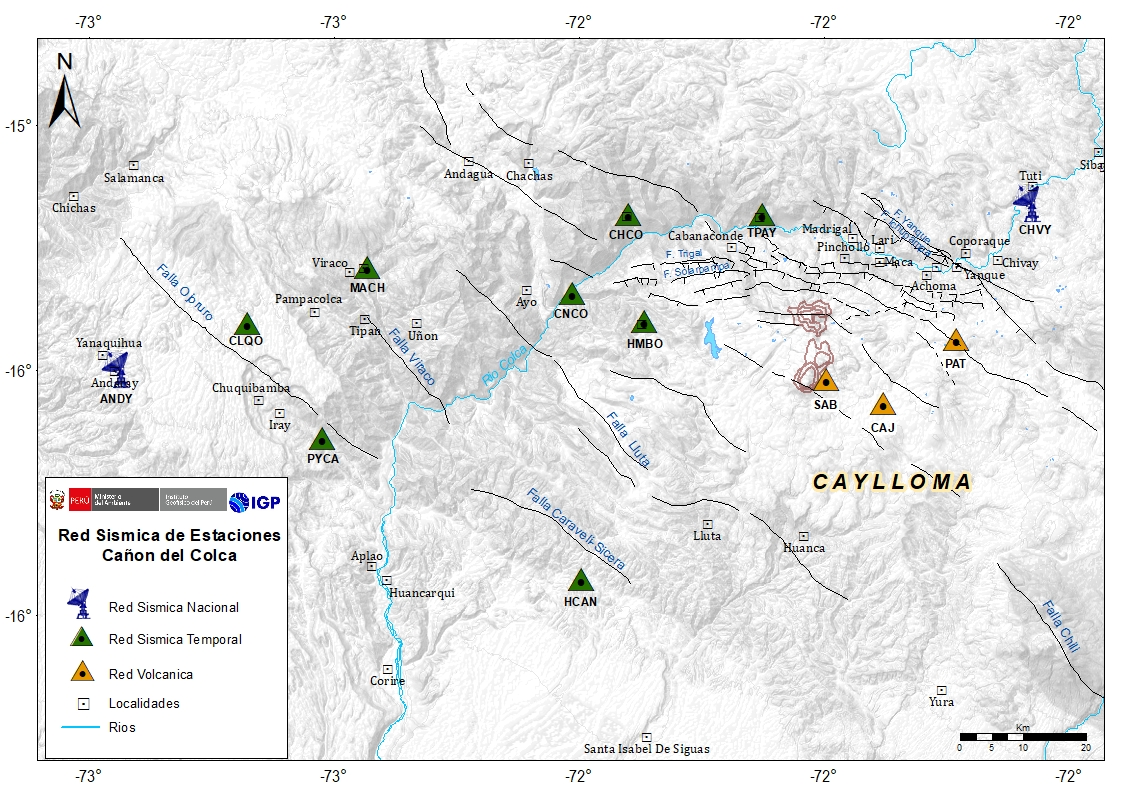
\includegraphics[width=1\linewidth]{images/red_colca}
 
\end{frame}

\begin{frame}
 
 {Historical large earthquakes: Valle del Colca}
 
 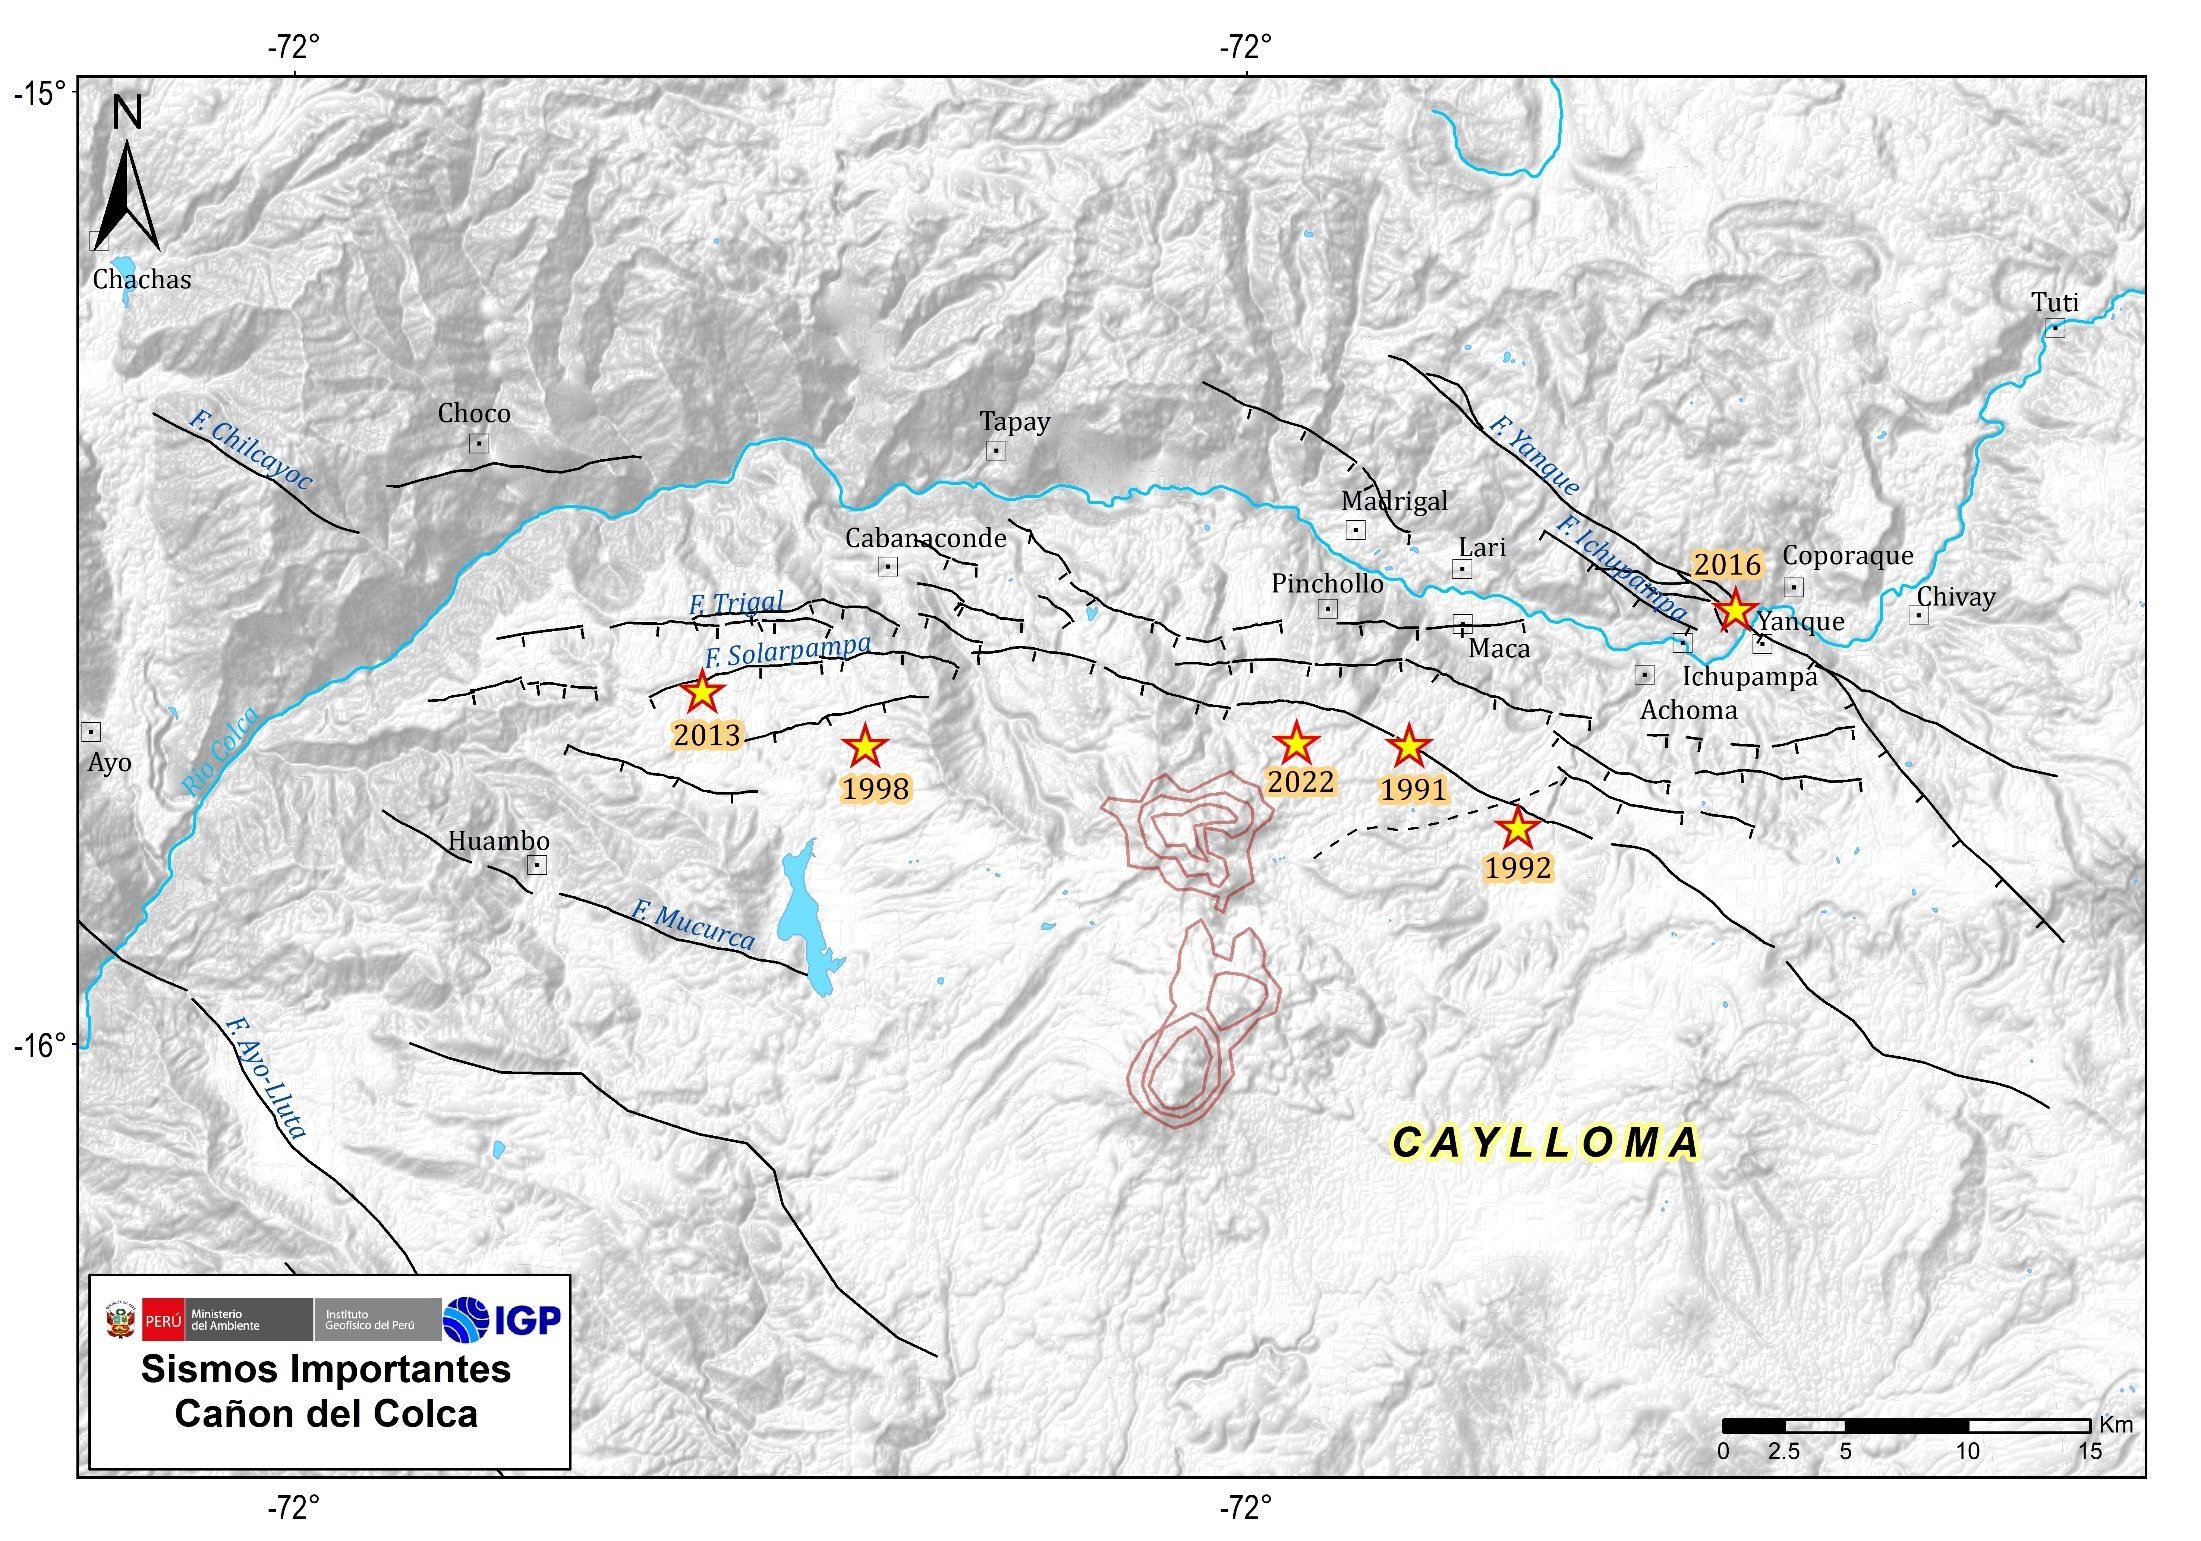
\includegraphics[width=1\linewidth]{images/red_colca_hist}
 
\end{frame}


\begin{frame}
 
 {Instrumented seismicity 2015-2021: Valle del Colca}
 
  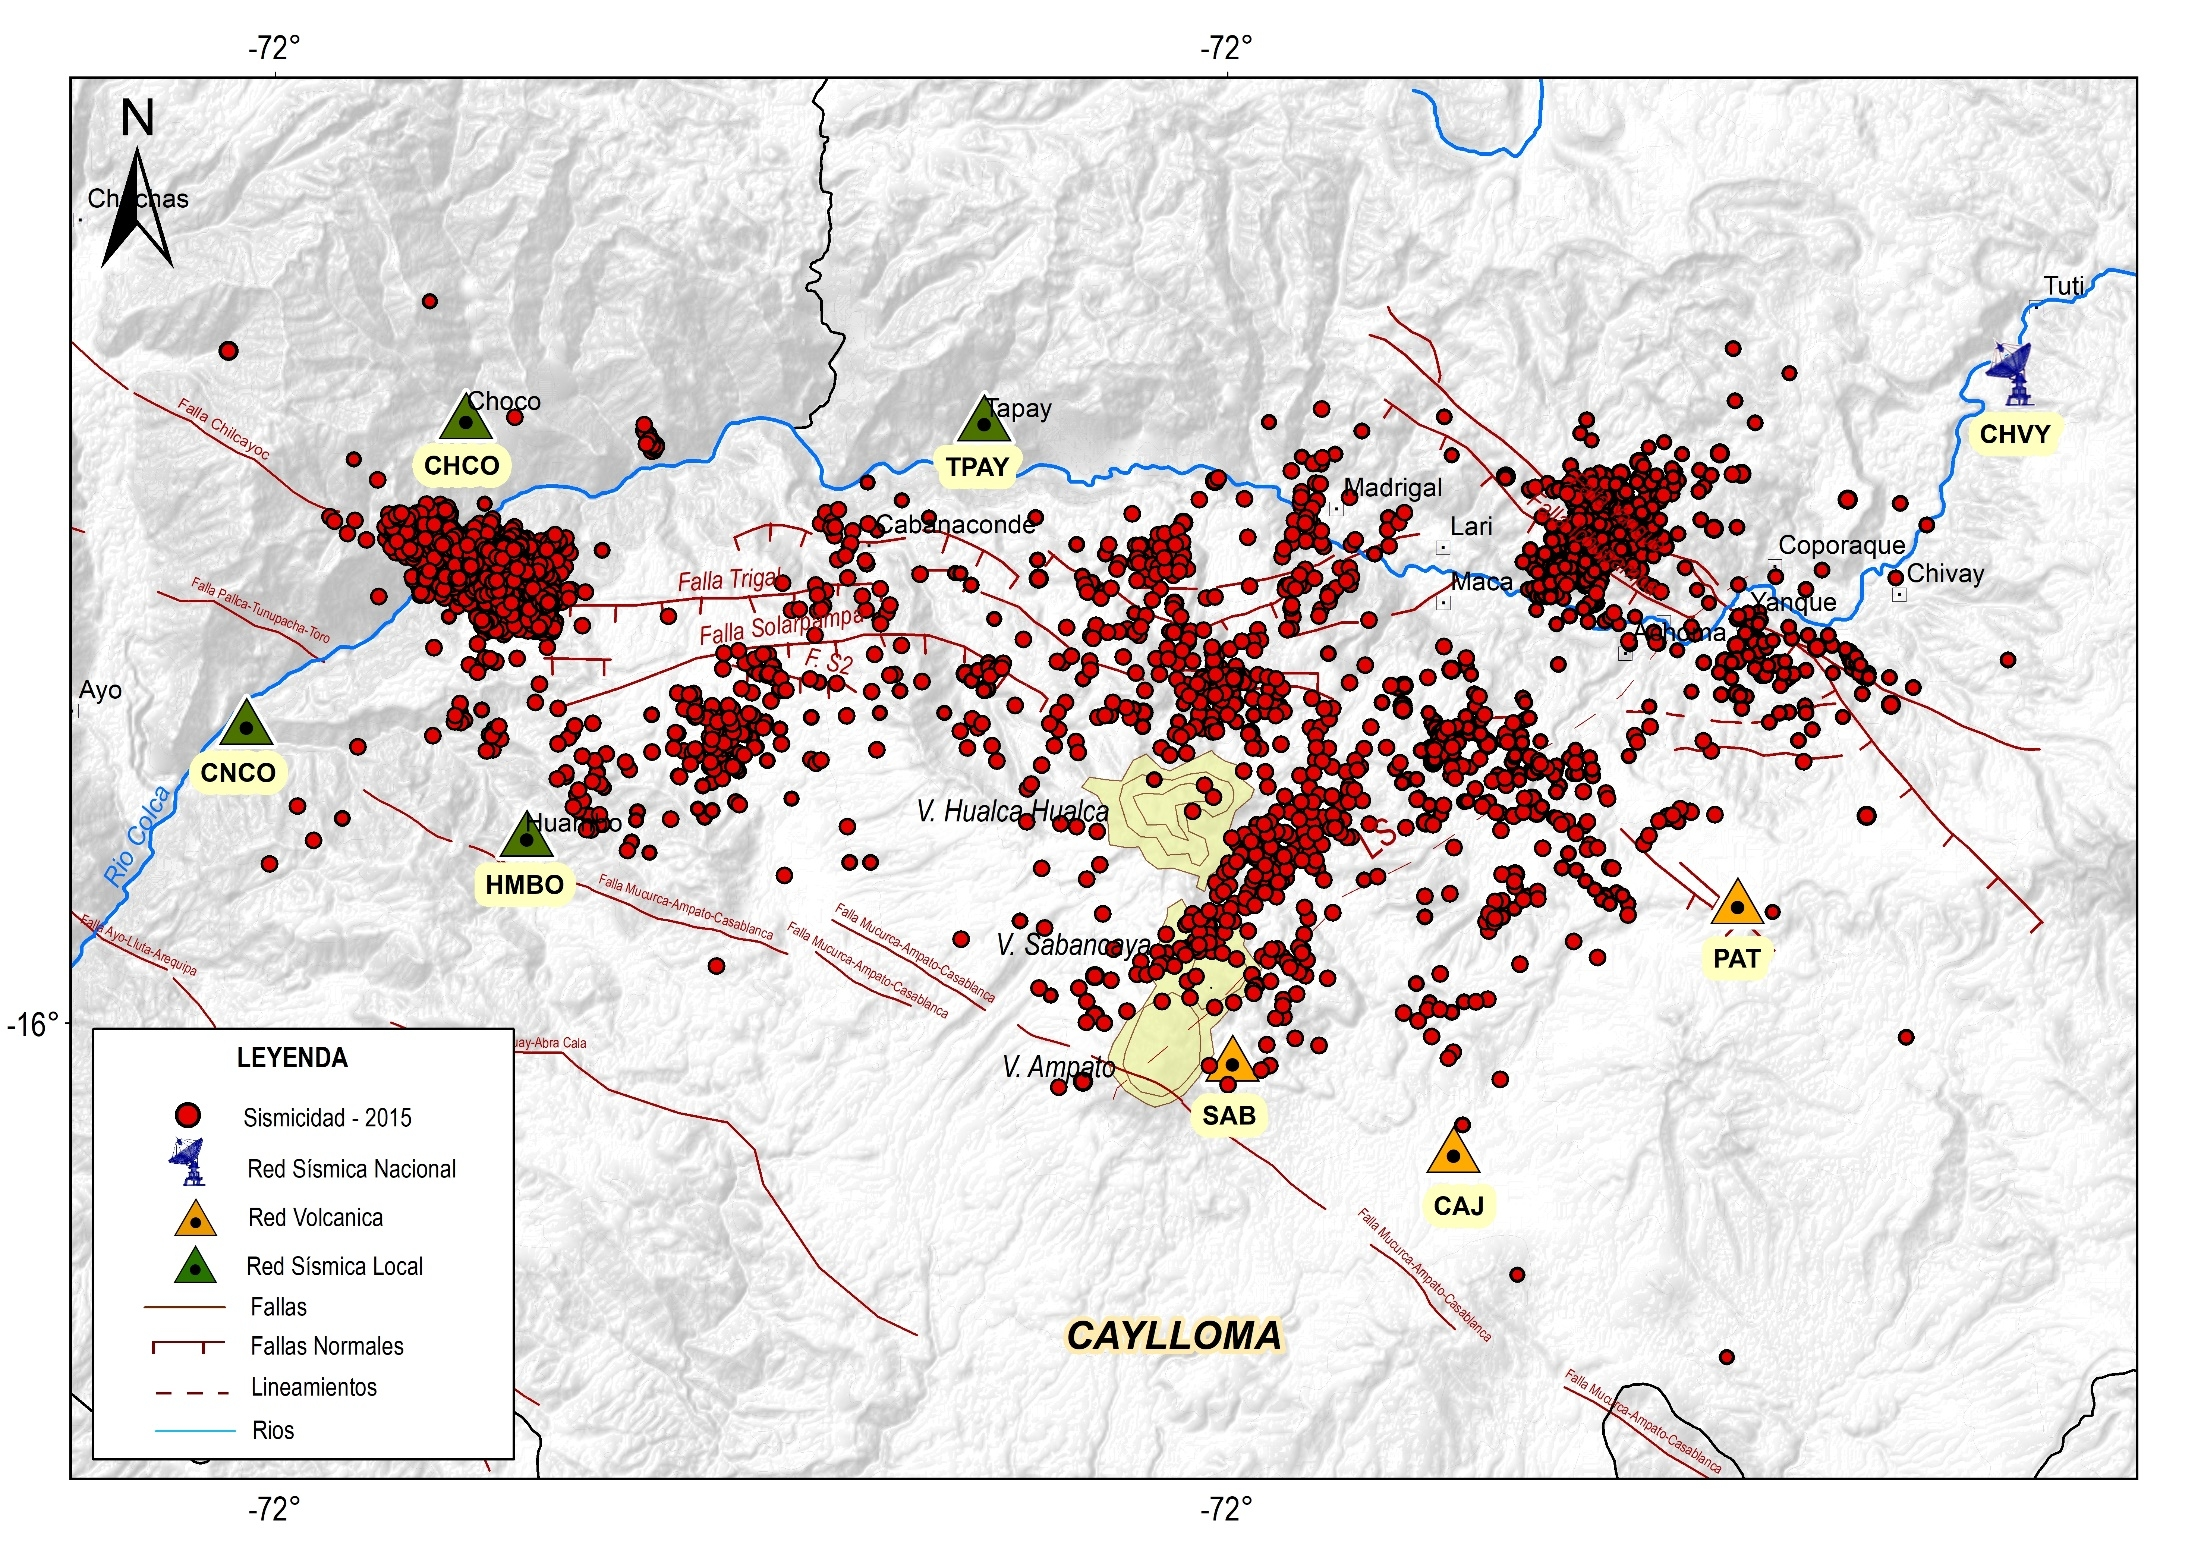
\includegraphics[width=1\linewidth]{images/red_colca_all}
 
\end{frame}


\begin{frame}
 
 {Well located large seismicity 2015-2021: Valle del Colca}
 
  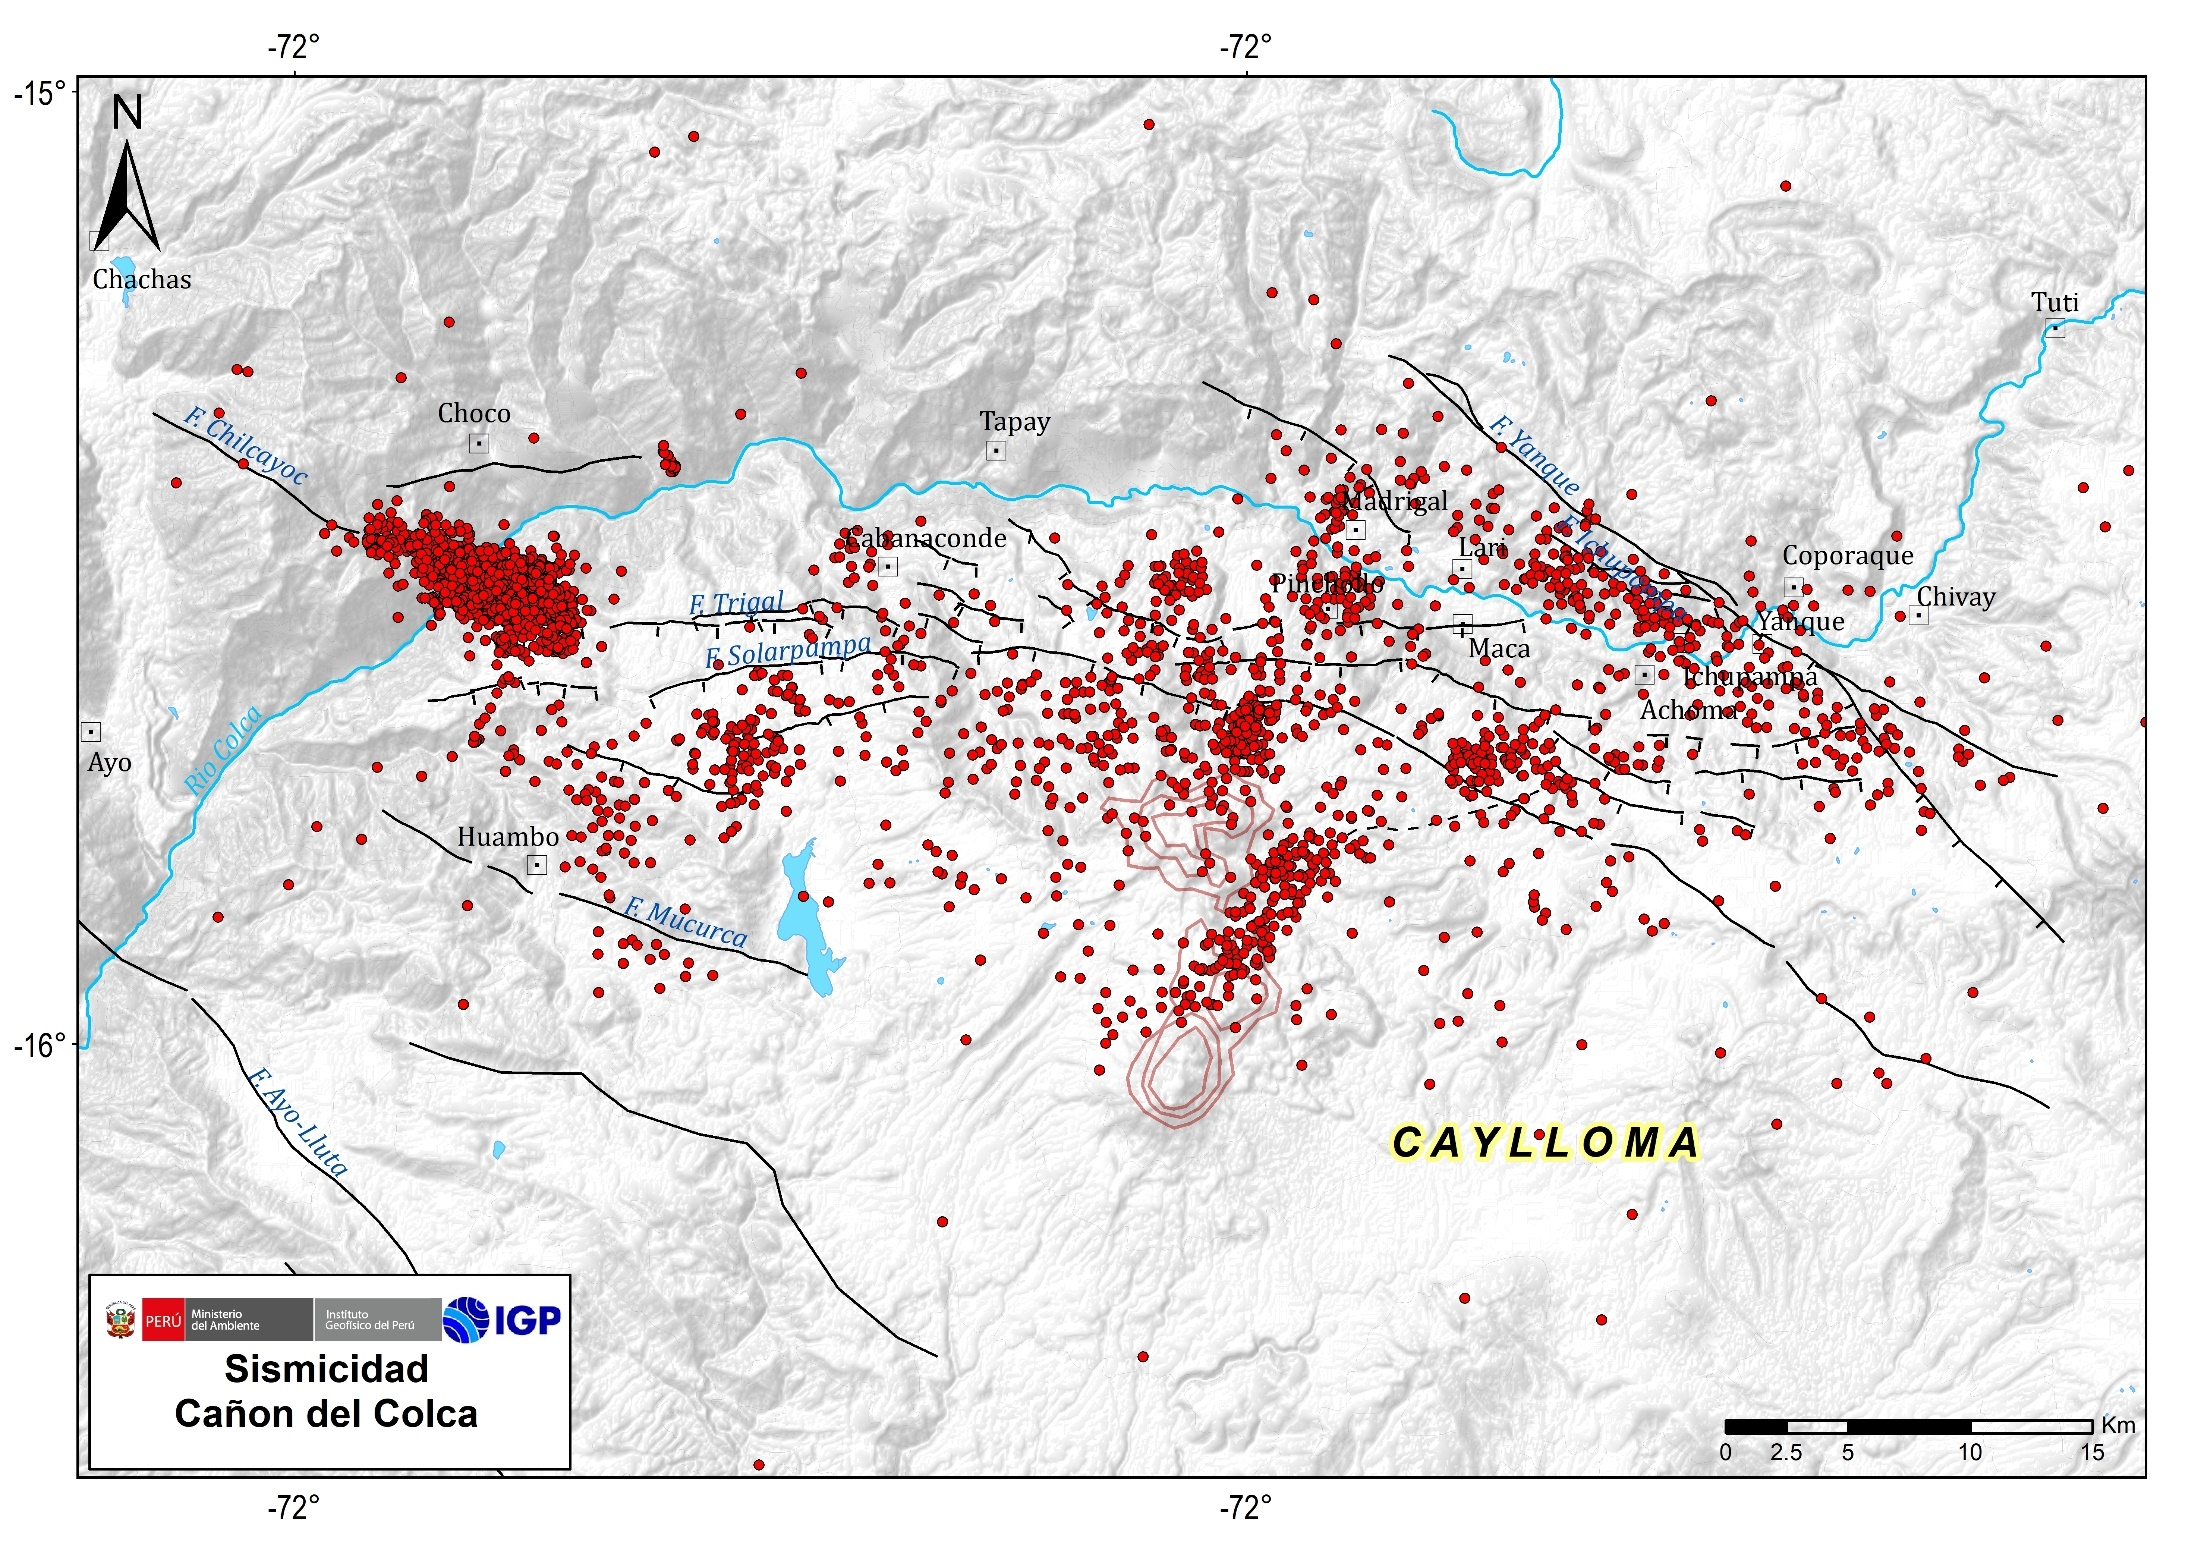
\includegraphics[width=1\linewidth]{images/red_colca_large}
 
\end{frame}


\end{document}

